%\documentclass[a4paper,12pt]{report} %размер бумаги устанавливаем А4, шрифт 12пунктов
\documentclass[a4paper,12pt, titlepage]{article}
%\usepackage[russian]{babel}   % включение переносов 
\usepackage{geometry}           % пакет для задания полей страницы командой \geometry
\geometry{left=3cm}% левое поле
\geometry{right=1.5cm}% правое поле
\geometry{top=2cm}% верхнее поле
\geometry{bottom=2cm}% нижнее поле

\usepackage[english,russian]{babel}
\usepackage[utf8]{inputenc}

\usepackage{amsmath}
%\usepackage{amsthm}
%\usepackage{cmap}
\usepackage{indentfirst}
\usepackage{a4wide,amssymb}
\usepackage{multicol} 
\usepackage{amssymb,amsfonts,amsmath,mathtext,cite,enumerate,float} %подключаем нужные пакеты расширений
\usepackage{longtable}
\tolerance=1000
\usepackage{graphicx}
%\usepackage[dvips]{graphicx} %хотим вставлять в диплом рисунки?
\graphicspath{{images/}}%путь к рисункам

%\usepackage[pdftex]{graphicx}
%\usepackage[pdftex]{graphics}
%\usepackage{wrapfig}
%\linespread{1.3}                % полтора интервала. Если 1.6, то два интервала
\pagestyle{plain}               % номерует страницы

\usepackage[usenames]{color}
 \usepackage{colortbl}

\renewcommand{\topfraction}{1}
\renewcommand{\textfraction}{0}


\begin{document}

\begin{titlepage}
\begin{center}
%Московский государственный университет им. М. В. Ломоносова\\
%Механико-математический факультет\\
%Кафедра вычислительной математики\\
МОСКОВСКИЙ ГОСУДАРСТВЕННЫЙ УНИВЕРСИТЕТ\\
им. М.В.ЛОМОНОСОВА\\
МЕХАНИКО-МАТЕМАТИЧЕСКИЙ ФАКУЛЬТЕТ
\end{center}
\vspace{1cm}
\begin{figure}[h]
\centering
\centerline{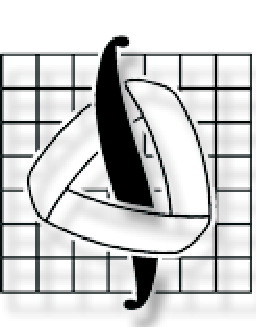
\includegraphics[height=3cm]{mebiusPDF.pdf}}
\end{figure}

\vspace{2cm}
\begin{center}
\large \bf{Дипломная работа}\\
студента 5 курса Калигина Н. Н.
\end{center}
\vspace{2cm}
\begin{center}
\LARGE \bf{Метод стандартного положения в задачах идентификации многогранников}
\end{center}

\vspace{3cm}

\large
\begin{flushright}
Научный руководитель: к. ф.-м. н. Валединский В. Д.
\end{flushright}

\vspace{2cm}

\begin{center}
Москва\\2012
\end{center}

\end{titlepage}

%\maketitle
\tableofcontents
%\begin{abstract}
%\end{abstract}

\newpage
\section{Введение}
\subsection{Происхождение вопроса}
С глубокой древности человека привлекали редкие минералы. В частности драгоценные камни.
Красота, долговечность и редкость -- главные достоинства драгоценного камня. 
Если редкость и долговечность присущи камням изначально,
то красивым внешним видом драгоценные камни, как правило, обладают только после полировки или огранки.

Драгоценные камни широко используют для производства ювелирных изделий, для промышленных нужд.  
Камни часто производят синтетическим путем. Значительное число добытых камней, цена и значимость изделий привели к тому, что 
появились различные их классификации и характеристики. Важна огранка камня, 
его чистота, цвет, вес в каратах, геометрические свойства.

При составлении документации для обработанного камня используют его схему (см. Рис. \ref{diamond}). На схеме
 изображен вид камня сбоку, вид сверху и вид внизу. При просмотре не возникает вопросов, почему выбраны именно такие 
ракурсы, точнее, почему выбранные ракурсы -- это вид сбоку, сверху и снизу. Нами интуитивно выбрана удобная система 
координат, потому что она удобна для описания огранки камня. При этом мы решили математическую задачу, в которой для 
многогранника нужно выбрать систему координат. Роль многогранника, соответственно, играл драгоценный камень. 
Стоит заметить, что необработанные камни тоже можно считать многогранниками. Правда, если у драгоценных камней после огранки 
может быть до 240 граней, то в необработанном камне их число может быть гораздо больше \cite{3dbook,wiki-ogranka}.   

\begin{figure}[h]
\noindent\centering{
    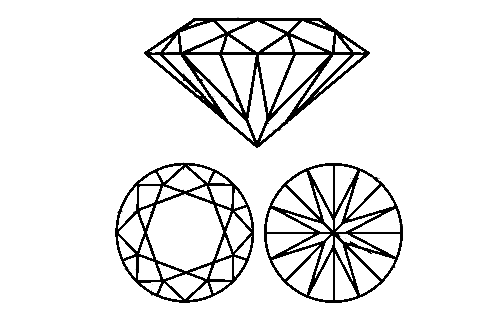
\includegraphics[clip,width=100mm]{diamond.png}
          }
\caption{Схематически изображенный бриллиант}
\label{diamond}
\end{figure}

\subsection{Постановка задачи}
Возникает следующая мысль. По какому-то определенному алгоритму, исходя из геометрических характеристик 
многогранника, найти для него систему координат, обладающую некоторыми свойствами. 

Во-первых, она жестко связана с многогранником, т.е. в этой системе координат многогранник всегда неподвижен.  

Во-вторых, система координат должна однозначно определяться с точностью до симметрий твердого тела. 

В-третьих, для двух похожих, но неравных тел, углы между соответствующими друг другу осями должны быть маленькими.
Другими словами, алгоритм должен внешне похожие камни ставить в одно и то же положение.

Такими системами координат мы можем охарактеризовать многогранник и сравнить два похожих многогранника. 
Но похожесть или не похожесть одного многогранника на другой -- это понятие субъективное, поэтому хотелось бы 
найти еще какие-нибудь наглядные характеристики, с которыми можно легко и эффективно работать. 

В частности, важно найти характеристику, которая позволяет сказать на сколько многогранники, поставленные в одно и
то же положение, отличаются друг от друга.


\subsection{Практическое применение}  
Огранка камней имеет большую историю. Первые формы обработки были достаточно примитивными, но в течение многих веков ювелиры 
разработали много таких огранок, что свет в драгоценных камнях максимально показывал всю гамму их оптических свойств. Со 
временем в этой области появилась своя терминология и стандарты. На Рис. \ref{diamond} изображен бриллиант с огранкой 
«Кр-57»\cite{Epif}.
В бриллианте можно чётко выделить две основные части: корона и павильон, их разделяет рундист. Вид сверху, это  вид на 
площадку(так называется большая грань бриллианта), смотря сбоку, мы площадку уже не увидим, она параллельна  плоскости нашего 
обзора. Оси координат однозначно мы определить в этом случае не можем, т.к. присутствуют симметрии в камне. Однако это не 
помешает нам наглядно описать огранку камня. 

Классификация по геометрическим свойствам драгоценного камня важна, как для обработанных, так и для необработанных экземпляров.
Огранка бриллианта зависит от формы исходного алмаза. При огранке алмазов стремятся минимизировать производственные потери. Вес 
бриллианта измеряют в каратах. Один карат это, приблизительно, 0,2 грамма. 
В мировой практике бриллианты подразделяют на мелкие -- до 0,29 
карата,  средние -- от 0,30 до 0,99 карата и крупные -- свыше 1 карата. Бывает, из одного алмаза выгодней сделать три средних, 
чем один крупный. При обработке алмазов, на основе фотографий строится 3D-модель. Как уже говорилось выше, необработанный камень 
может быть представлен в виде многогранника с очень большим числом граней. Расчет того, какие именно бриллианты делать из алмаза, 
может быть быть довольно трудоемкий, поэтому, если нам удастся идентифицировать кристалл, как ранее обработанный, то эти расчеты 
повторно проводить не нужно.  


\newpage
\section{Простые геометрические характеристики многогранника}

\begin{figure}[h]
\noindent
\begin{multicols}{2}
\noindent\centering{
    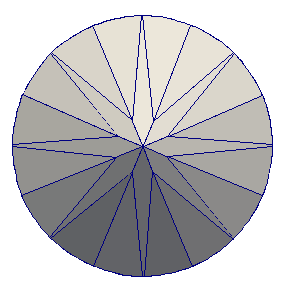
\includegraphics[clip,width=50mm]{brill_z_minus.png}          
}		
	\caption{Вид снизу}
	\label{brill_z_minus}

\noindent\centering{
    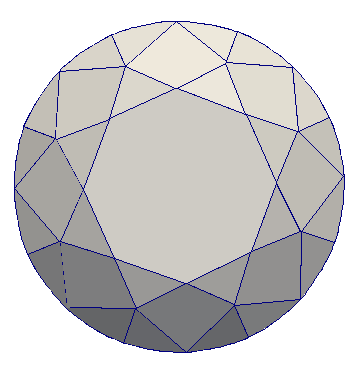
\includegraphics[clip,width=50mm]{brill_z_plus.png}
}		
	\caption{Вид сверху}
	\label{brill_z_plus}
\end{multicols}
\end{figure}

\begin{figure}[h]
\noindent\centering{
    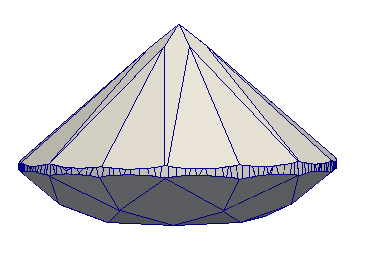
\includegraphics[clip,width=75mm]{brill_x_plus.png}
          }
\caption{Вид сбоку}
\label{brill_x_plus}
\end{figure}
В качестве опытных образцов возьмем семь трехмерных моделей алмазов, с огранкой «Кр-57», подобных, 
изображенному на Рис. \ref{brill_z_minus}-\ref{brill_x_plus}. Несмотря на стандартное количество граней в 
огранке, рундист и сколы камня увеличивают число граней в многограннике. В используемых образцах в среднем около
250-300 граней и 500-600 вершин. Перед нами встает выбор, какие характеристики многогранника использовать для решения 
поставленной задачи и какие из них наиболее точно смогут идентифицировать многогранник в реальных условиях.
 
\subsection{Точечные характеристики}
Очевидным образом можно задать многогранник с помощью его вершин и ребер. Можно пользоваться такими характеристиками
многогранника, как координаты его вершин, длины ребер и их углы между собой. Многогранник в таком случае будет отождествлен 
со своеобразным каркасом. На нем можно произвольным образом выбрать точки (к примеру вершины и с заданным интервалом точки на 
рёбрах). В таком случае многогранник превращается в множество заданного количества точек. Попытаемся для такого множества выбрать 
систему отсчета. В качестве начала системы отсчета можно взять естественную физическую характеристику -- центр масс. Положение 
центра масс системы материальных точек в классической механике определяется следующим образом: 
$$\vec r_{c} = \frac{\sum\limits_{i} {\vec {r}_{i}}{m}_{i}}{\sum\limits_{i} {m}_{i}}$$
$\vec r_{c}$ -- радиус-вектор центра масс, $\vec r_{i}$ -- радиус-вектор $i$-й точки системы, $\vec m_{i}$ -- масса $i$-й точки.
Можно считать, что все точки весят одинаково, а их суммарная масса равна 1.
При выборе направления осей возникают проблемы. Мы можем исходить из координат точек, из их расстояний между собой, но 
нужно помнить, что данную модель мы строим для работы с твердыми телами. При добавлении или удалении точек из системы, эта 
система меняется. Для большего числа используемых точек эти изменения менее заметны, поэтому имеет смысл в качестве 
характеристик, идентифицирующих многогранник, использовать поверхностные и объемные характеристики. В таких моделях 
погрешность измерений будет компенсироваться числом точек. Так, например, центр масс, который мы будем использовать в дальнейшем,
рассчитан тем достовернее, чем больше точек в системе, особенно, 
если выбирать точки не только на ребрах, а по всему многограннику
и его поверхности. Но использование большого числа промежуточных точек, загружает систему. Тем более, знать и хранить информацию
о каждой точке в принципе не обязательно. Наиболее важна их совокупная характеристика.   

\subsection{Площадь поверхности}
Площадь поверхности многогранника слабо меняется при малом сдвиге какой-то точки. Она мало меняется при добавлении 
лишней грани (добавление лишней грани может произойти при получении трехмерной модели камня фотографированием его 
теневых контуров при вращении камня на подставке). Нахождение площади поверхности представляет интерес для решения поставленной 
задачи. 

Найдем площадь каждой грани и сложим их.  Нам известны координаты всех 
вершин многогранника в трехмерном пространстве, количество этих вершин. Известны грани. Грань описана списком вершин,
которые  в неё входят, и плоскостью, в которой эти вершины лежат(плоскость при этом задается четырьмя своими 
 коэффициентами $a$, $b$, $c$, $d$ из уравнения плоскости $a x + b y + c z + d = 0$). 
Наши многогранники ориентированны \cite{zor} , т.е. задано направление, в котором обходятся вершины каждой грани.

\begin{figure}[h]
\noindent\centering{
    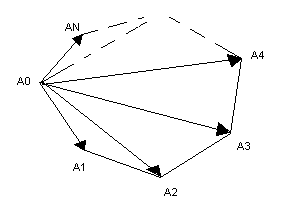
\includegraphics[clip,width=70mm]{sarea.png}
          }
\caption{Нахождение ориентированной площади}
\label{sarea}
\end{figure}

Площадь каждой грани будем искать следующим образом.
\begin{enumerate}
\item Выберем первую вершину $A_{0}$ из списка вершин и отложим из нее два вектора $\overrightarrow{A_{0}A_{1}}$ 
и $\overrightarrow{A_{0}A_{2}}$ в две следующие за первой вершины.
\item Найдем ориентированную площадь треугольника, лежащего между двумя построенными векторами, как половину
векторного произведения этих векторов.
Так проделаем для каждого ребра грани (т.е векторов $\overrightarrow{A_{0}A_{i}}$ 
и $\overrightarrow{A_{0}A_{i+1}}$), кроме тех, которым принадлежит первая вершина. 
\item Сложим полученные ориентированные площади.
\end{enumerate}

Этим методом можно найти площадь не только выпуклого многоугольника, но и невыпуклого. Для невыпуклого многогранника 
не все ориентированные площади будут положительны, будут  и отрицательные, но равные по модулю им положительные площади 
при этом войдут несколько раз. Поэтому в итоге мы получим исходную площадь  многоугольника. Сложив все площади граней, получим
искомую площадь поверхности. Для семи многогранников, о которых говорилось в начале, составлена следующая таблица:
 

%\begin{center}
%\begin{tabular}{|c|c|}
%\hline
%№ & Площадь поверхности\\
%\hline
%1 & 70.23062416384944128822098718956112861633300781250000\\
%\hline
%2 & 80.96629778007144295770558528602123260498046875000000\\
%\hline
%3 & 85.23628106051681641019968083128333091735839843750000\\
%\hline
%4 & 86.40407086488922061562334420159459114074707031250000\\
%\hline
%5 & 98.73665902982818920463614631444215774536132812500000\\
%\hline
%6 & 98.73059348637481491550715873017907142639160156250000\\
%\hline
%7 & 98.73783243369690865165466675534844398498535156250000\\
%\hline  
%\end{tabular}
%\end{center}

\begin{center}
\begin{tabular}{|p{0.5cm}|p{2.4cm}|p{12cm}|}
\hline
№ & Площадь поверхности & Название\\
\hline
1 & 70.2306 & 2009 08 06 round 0 76ct Lexus Radius no 1 no 5 missing RBC 2\\
\hline
2 & 80.9662 & 2009 08 06 round 0 93ct Lexus Radius no 1 no 5 missing RBC 1\\
\hline
3 & 85.2362 & 2009 08 06 round 1 01ct Lexus Radius no 1 no 5 missing RBC 3\\
\hline
4 & 86.4040 & 2009 08 06 round 1 04ct Lexus Radius no 1 no 5 missing RBC 4\\
\hline
5 & 98.7366 & 2009 08 17 brilliant 1.27ct lexus 400c wol 2\\
\hline
6 & 98.7305 & 2009 08 17 brilliant 1.27ct lexus 400c wol 3\\
\hline
7 & 98.7378 & 2009 08 17 brilliant 1.27ct lexus 400c Wol 1\\
\hline  
\end{tabular}
\end{center}


На данном этапе мы брали совокупную площадь всех граней. Если же объединять площади не всех граней сразу, 
а определенных групп, то можно выделить на многограннике определенные участки. В ювелирном деле такие участки имеют 
сложившиеся названия: рундист, корона, павильон, площадка. Заметим, что у камней с одинаковой огранкой и весом
площади этих участков будут совпадать.

Если площади поверхностей двух многогранников не совпадают, то мы можем различить их по площади. Если же площади
совпадают, то необходимо продолжить исследование многогранников. Так например выше в таблице наиболее интересные 
для исследования многогранники с номерами 5-7, так как у них наблюдается совпадение до сотых в значениях площадей
их поверхностей.  
 
\subsection{Объем}
Объем многогранника -- еще менее чувствительная к появлению лишней вершины или ребра характеристика многогранника.
Для поиска объема многогранника  воспользуемся понятиями ориентированного объема и смешанного произведения.

Наши многогранники ориентированны, т.е. задано направление, в котором обходятся вершины каждой грани.
Объем всего многогранника, мы найдем как сумму ориентированных объемов пирамид, в основании которых 
лежат грани нашего многогранника. Ориентированный объем каждой из пирамид -- это сумма ориентированных 
объемов тетраэдров, основаниями которых являются треугольники, используемые для нахождения площади поверхности.

\begin{figure}[h]
\noindent\centering{
    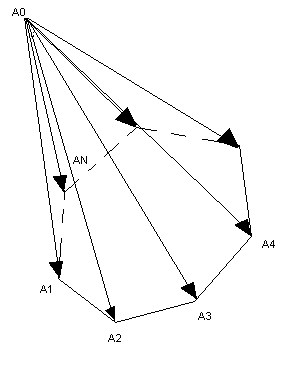
\includegraphics[clip,width=70mm]{vol.png}
          }
\caption{Нахождение ориентированного объема}
\label{vol}
\end{figure}

\newpage
Объем каждой пирамиды будем искать следующим образом.
\begin{enumerate}
\item Выберем точку $A_{0}$ вне многогранника. При решении задачи выбиралась точка на оси $Oz$, 
аппликата которой на единицу больше, чем аппликата любой из вершин многогранника.
\item Выберем первую вершину из списка вершин грани $A_{1}$. 
\item Выберем две вершины $A_{2}$ и $A_{3}$, следующие за $A_{1}$.
\item Найдем ориентированную площадь тетраэдра $A_{0}A_{1}A_{2}A_{3}$, как одну шестую смешанного векторного произведения
$(\overrightarrow{A_{0}A_{1}},\overrightarrow{A_{0}A_{2}},\overrightarrow{A_{0}A_{3}})$. 
\item Так проделаем для каждого тетраэдра $A_{0}A_{1}A_{i}A_{i+1}$ грани.
\item Сложим полученные ориентированные площади тетраэдров.
\end{enumerate}


%\begin{center}
%\begin{tabular}{|c|c|}
%\hline
%№ & Объем\\
%\hline
%1 & 43.24525406686564821256979485042393207550048828125000\\
%\hline
%2 & 52.96440575160323760428582318127155303955078125000000\\
%\hline
%3 & 57.56587209039060581972080399282276630401611328125000\\
%\hline
%4 & 59.21963211339889454620788455940783023834228515625000\\
%\hline
%5 & 72.12884038836051558973849751055240631103515625000000\\
%\hline
%6 & 72.12171319957417381374398246407508850097656250000000\\
%\hline
%7 & 72.12903930501069282854587072506546974182128906250000\\
%\hline 
%\end{tabular}
%\end{center}

\begin{center}
\begin{tabular}{|p{0.5cm}|p{2.4cm}|p{12cm}|}
\hline
№ & Объем & Название\\
\hline
1 & 43.2452 & 2009 08 06 round 0 76ct Lexus Radius no 1 no 5 missing RBC 2\\
\hline
2 & 52.9644 & 2009 08 06 round 0 93ct Lexus Radius no 1 no 5 missing RBC 1\\
\hline
3 & 57.5658 & 2009 08 06 round 1 01ct Lexus Radius no 1 no 5 missing RBC 3\\
\hline
4 & 59.2196 & 2009 08 06 round 1 04ct Lexus Radius no 1 no 5 missing RBC 4\\
\hline
5 & 72.1288 & 2009 08 17 brilliant 1.27ct lexus 400c wol 2\\
\hline
6 & 72.1217 & 2009 08 17 brilliant 1.27ct lexus 400c wol 3\\
\hline
7 & 72.1290 & 2009 08 17 brilliant 1.27ct lexus 400c Wol 1\\
\hline  
\end{tabular}
\end{center}


В таблице указаны посчитанные объемы семи многогранников. Объем представляет аналогичную площади поверхности характеристику.
Для двух многогранников сигналом несовпадения или возможного совпадения может служить объем. В таблице у 
многогранников с номерами 5-7, наблюдается совпадение до сотых в значениях объема, как  это было с величинами 
площадей их поверхностей. 

Объем и площадь поверхности сами по себе довольно слабые характеристики, т.к. явно они могут сказать только или о сильном несовпадении двух многогранников или о том, что два многогранника предположительно совпадают. Ниже будет описано, как с помощью
площади поверхности и объема получить более сильные характеристики.

\newpage

\section{Оси инерции}
\subsection{Начальные определения}
Одну из наиболее ярких характеристик твердого тела мы можем взять из курса теоретической механики. 
Это тензор инерции\cite{vilke}. 

Пусть твердое тело вращается вокруг неподвижной точки $O$. В нашем случае это будет центр масс, о котором говорилось выше,
но сейчас мы пересчитаем его, используя описанный алгоритм нахождения объема через смешанное векторное произведение.
Примем эту точку за начало системы координат $O\xi_{1}\xi_{2}\xi_{3}$. Если $\Omega$ мгновенная угловая скорость тела,
то момент количеств движения $G$ и кинетическая энергия $T$ определяются следующими формулами
$$G = \int \limits_{\Omega}[r,\dot{r}]d\mu = \int \limits_{\Omega}[r,[\Omega,r]]d\mu$$  

$$2T = \int \limits_{\Omega} \dot{r}^{2} d\mu = \int \limits_{\Omega} [\Omega,r]^{2}d\mu$$  

Из этих формул в частности вытекает равенство $2T = G\Omega$. 

Проекции радиус-вектора $r$ и  вектора мгновенной угловой скорости 
$\Omega$ обозначим через $({\Omega}_{1},{\Omega}_{2},{\Omega}_{3})$, $({\xi}_{1},{\xi}_{2},{\xi}_{3})$, 
получим 
$$2T = \int \limits_{\Omega}\left[ (   \Omega_{2}\xi_{3} - \Omega_{3}\xi_{2})^{2} 
									+ (\Omega_{3}\xi_{1} - \Omega_{1}\xi_{3})^{2} 
									+ (\Omega_{1}\xi_{2} - \Omega_{2}\xi_{1})^{2} \right]d\mu = $$
									
$$
 = {J}_{11}{\Omega}_{1}^{2} + {J}_{22}{\Omega}_{2}^{2} +{J}_{33}{\Omega}_{3}^{2}
 - 2{J}_{12}{\Omega}_{1}{\Omega}_{2} - 2{J}_{23}{\Omega}_{2}{\Omega}_{3} - 2{J}_{13}{\Omega}_{1}{\Omega}_{3},
$$
$$
{J}_{ii} = \int \limits_{\Omega} ({r}^{2} - {\xi}_{i}^{2})d\mu,\;\;\;\;{J}_{ij}  = \int \limits_{\Omega}\xi_{i}\xi_{j}d\mu,
\;\;\;\; i \neq j. 
$$

Величина ${J}_{ii}$ называется моментом инерции тела относительно оси $O\xi_{i}$, а центробежным моментом инерции называется
величина ${J}_{ij}\;(i \neq j)$. Квадратичная форма представима в виде $2T =  (J\Omega,\Omega)$.
Симметричный тензор инерции тела в системе координат $O\xi_{1}\xi_{2}\xi_{3}$, или оператор инерции выглядит следующим образом
\[
J = 
\begin{Vmatrix}
{J}_{11} & -{J}_{12} & -{J}_{13}\\
-{J}_{12} & {J}_{22} & -{J}_{23}\\
-{J}_{13} & -{J}_{23} & {J}_{33}\\
\end{Vmatrix}
\]
\newpage
\subsection{Вычисление тензора инерции и центра масс}
Ортогональным преобразованием мы можем привести Тензор инерции к главным осям. В главных осях центробежные моменты
инерции равны нулю.

Остановимся на ряде свойств тензора инерции:
\begin{enumerate}
\item Задача отыскания главных осей инерции совпадает с задачей определения собственных векторов оператора инерции, 
когда справедливо соотношение $J\omega = \lambda\omega$, и совпадает с задачей отыскания условного экстремума 
кинетической энергии на сфере ${S}^{2} = \{\omega:\omega^{2}  = 1\}$.
\item Главные моменты инерции являются корнями характеристического уравнения ${\rm det}\|J - \lambda E\| = 0$.
\item Собственные векторы, отвечающие различным корням $\lambda_{k}$ характеристического уравнения, ортогональны, а  
корни $\lambda_{k}$ вещественны. 
\end{enumerate}

Таким образом, задачу приведения тензора инерции к главным осям можно решить, учитывая симметричность тензора, итерационным 
методом Якоби для вычисления собственных значений и собственных векторов вещественной симметричной матрицы.

Вычисление тензора инерции сводится к вычислению по формулам, написанным выше, диагональных и не диагональных его компонент:
\begin{center}
$J_{xx} = \iiint \limits_V (y^2 +  z^{2})\,dxdydz$ - пример диагональной компоненты,

$J_{xy} = - \iiint \limits_V (xy)\,dxdydz$ - пример не диагональной компоненты.
\end{center}

Компоненты нужно вычислить по всему объему, но сделать это довольно проблематично. Поэтому мы поступим, как в алгоритме 
вычисления объема многогранника. Выберем точку вне многогранника и для каждой грани найдем величину интеграла, посчитанного
по ориентированному объему пирамиды, основанием которой является выбранная грань. Причем интеграл по объему пирамиды найдем,
как сумму интегралов по ориентированным объемам тетраэдров, составляющих пирамиды. 

Тройной интеграл по тетраэдру мы вычислим следующим образом. Построим аффинное преобразование между тетраэдром, 
который нам известен, чтобы считать тройной интеграл не по произвольному объему, а по известному. Тетраэдр $T$ задан в
системе координат $Oxyz$ точкой $A({x}_{0},{y}_{0},{z}_{0})$, которую мы выбрали вне многогранника, и 
тремя векторами $\vec u$, $\vec v$ и $\vec w$. 
Аффинное преобразование сопоставит тетраэдр $T'$ в системе координат $Ox'y'z'$ и тетраэдр $T$,
причем вершина $A$ соответствует $(0,0,0)$, вектор $\vec u$ соответствует вектору $(1,0,0)$, 
вектор $\vec v$ вектору $(0,1,0)$, вектор $\vec w$ вектору $(0,0,1)$.  

\begin{figure}[h]
\noindent\centering{
    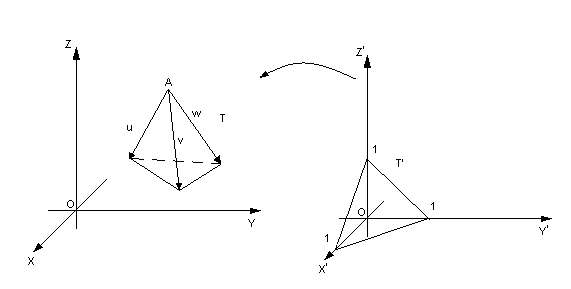
\includegraphics[clip,width=130mm]{taff.png}
          }
\caption{Аффинное преобразование тетраэдра}
\label{taff}
\end{figure}
\newpage

Итак $\vec u = ({u}_{x},{u}_{y},{u}_{z})$, $\vec v = ({v}_{x},{v}_{y},{v}_{z})$, $\vec w = ({w}_{x},{w}_{y},{w}_{z})$.
Произведем замену:
$$x = x(x',y',z')\;\;\;\;x(0,0,0) = x_0$$
$$y = y(x',y',z')\;\;\;\;y(0,0,0) = y_0$$
$$z = z(x',y',z')\;\;\;\;z(0,0,0) = z_0$$

\[
 	\left\{
 		\begin{aligned}
			x = x_0 + u_x x' + v_x y' + w_x z'\\
			y = y_0 + u_y x' + v_y y' + w_y z'\\
			z = z_0 + u_z x' + v_z y' + w_z z'\\
		\end{aligned}
	\right.
\]

\subsubsection{Вычисление тензора инерции}
И подсчет компонент тензора инерции сводится к подсчету интегралов вида 

\begin{center}
$I_{1} = \iiint \limits_T {x}^2 \,dxdydz $ 
и
$
I_{2} = \iiint \limits_T xy \,dxdydz
$
\end{center}

$$
I_{1} = \iiint \limits_T {x}^2 \,dxdydz 
= {\rm detJ} \int \limits_{0}^{1}~dz \int \limits_{0}^{1-z}~dx \int \limits_{0}^{1-z-x}~dy\;\;(x_0 + u_x x' + v_x y' + w_x z')^2 =$$
$$
= {\rm detJ} \int \limits_{0}^{1}~dz \int \limits_{0}^{1-z}~dx \int \limits_{0}^{1-z-x}~dy
(x_0^2 + u_x^2 x^2 + v_x^2 y^2 + w_x^2 z^2 + 2x_0 u_x x + 2 x_0 v_x y +$$
$$+  2 x_0 w_x z + 2 u_x v_x xy 
+ 2u_x w_x xz + 2v_x w_x yz)^2 = {\rm detJ} \sum \limits_{i = 1}^{10} K_i$$

Где $K_i$ это интегралы, соответствующие элементам суммы подынтегрального выражения, а ${\rm detJ}$ якобиан замены координат.
Якобиан находим, как смешанное произведение векторов, выходящих из выбранной точки вне многогранника в его вершины. Для тетраэдра,
изображенного на Рис. \ref{taff} якобиан ${\rm detJ} = (u,v,w) = ([u,v],w)$.

$$K_1 = \frac{1}{6}x_0^2\;\;\;K_2 = \int \limits_{0}^{1}~dz \int \limits_{0}^{1-z}~dx \int \limits_{0}^{1-z-x}~dy\;\;u_x^2 x^2 = 
u_x^2 \int \limits_{0}^{1}~dz \int \limits_{0}^{1-z}(1-z-x)dx =$$
$$
= u_x^2 \int \limits_{0}^{1}~dz \left.\left[ (1-z)\frac{x^3}{3} - \frac{x^4}{4}\right] \right|^{1-z}_{0}  
= u_x^2 \int \limits_{0}^{1}\frac{(1-z)^4}{12}dz = \frac{u_x^2}{60}
$$ 
$$K_3 = \int \limits_{0}^{1}~dz \int \limits_{0}^{1-z}~dx \int \limits_{0}^{1-z-x}~dy\;\;v_x^2 y^2 = \frac{v_x^2}{60}$$
$$K_4 = \int \limits_{0}^{1}~dz \int \limits_{0}^{1-z}~dx \int \limits_{0}^{1-z-x}~dy\;\;w_x^2 z^2 = \frac{w_x^2}{60}$$
$$K_5 = \int \limits_{0}^{1}~dz \int \limits_{0}^{1-z}~dx \int \limits_{0}^{1-z-x}~dy\;\;2x_0 u_x x 
= 2x_0 u_x x \int \limits_{0}^{1}~dz \int \limits_{0}^{1-z}x(1-z-x)dx =$$
$$
= 2x_0 u_x x \int \limits_{0}^{1}~dz \left.\left[ (1-z)\frac{x^2}{2} - \frac{x^3}{3}\right] \right|^{1-z}_{0}
= 2x_0 u_x \int \limits_{0}^{1}\frac{(1-z)^3}{6}dz = \frac{x_0 u_x}{12}$$
$$K_6 = \int \limits_{0}^{1}~dz \int \limits_{0}^{1-z}~dx \int \limits_{0}^{1-z-x}~dy\;\; 2x_0 v_x y = \frac{x_0 v_x}{12}$$
$$K_7 = \int \limits_{0}^{1}~dz \int \limits_{0}^{1-z}~dx \int \limits_{0}^{1-z-x}~dy\;\; 2x_0 w_x z = \frac{x_0 w_x}{12}$$
$$K_8 = \int \limits_{0}^{1}~dz \int \limits_{0}^{1-z}~dx \int \limits_{0}^{1-z-x}~dy\;\; 2u_x v_x xy
= u_xv_x\int \limits_{0}^{1}~dz \int \limits_{0}^{1-z}x(1-z-x)^2dx =$$
$$
= u_x v_x\int \limits_{0}^{1}~dz \int \limits_{0}^{1-z}~dx\left[ x(1-z)^2 - 2x^2(1-z) + x^3\right] =$$
$$
= u_x v_x\int \limits_{0}^{1}~dz \left.\left[ (1-z)^2\frac{x^2}{2} - \frac{2x^3}{3}(1-z) + \frac{x^4}{4}\right] \right|^{1-z}_{0}
= u_x v_x\int \limits_{0}^{1}\frac{z^4}{12} dz = \frac{u_x v_x}{60}$$
$$K_9 = \frac{u_x w_x}{60}\;\;\;\;\;K_{10} = \frac{v_x w_x}{60}$$

Таким образом, мы нашли слагаемые, которые составляют моменты инерции тел относительно осей координат 
$$ J_{xx} = J_{y} + J_{z}\;\;\;\;\;J_{yy} = J_{x} + J_{z}\;\;\;\;\;J_{zz} = J_{x} + J_{y},\text{ где}$$

$$
J_x =\iiint \limits_T {x}^2 \,dxdydz = {\rm detJ}\left( \frac{1}{6}x_0^2 
+ \frac{u_x^2}{60} + \frac{v_x^2}{60} + \frac{w_x^2}{60} +\right.
$$

$$
\left. + \frac{x_0 u_x}{12} + \frac{x_0 v_x}{12} + \frac{x_0 w_x}{12}
+ \frac{u_x v_x}{60} + \frac{u_x w_x}{60} + \frac{v_x w_x}{60}
\right)
$$

$$
J_y =\iiint \limits_T {y}^2 \,dxdydz = {\rm detJ}\left( \frac{1}{6}y_0^2 
+ \frac{u_y^2}{60} + \frac{v_y^2}{60} + \frac{w_y^2}{60} +\right.
$$
$$
\left.+ \frac{y_0 u_y}{12} + \frac{y_0 v_y}{12} + \frac{y_0 w_y}{12}
+ \frac{u_y v_y}{60} + \frac{u_y w_y}{60} + \frac{v_y w_y}{60}
\right)
$$
$$
J_z =\iiint \limits_T {z}^2 \,dxdydz = {\rm detJ}\left( \frac{1}{6}z_0^2 
+ \frac{u_z^2}{60} + \frac{v_z^2}{60} + \frac{w_z^2}{60} +\right.
$$
$$
\left.+ \frac{z_0 u_z}{12} + \frac{z_0 v_z}{12} + \frac{z_0 w_z}{12}
+ \frac{u_z v_z}{60} + \frac{u_z w_z}{60} + \frac{v_z w_z}{60}
\right)
$$

Посчитаем интегралы для центробежных моментов инерции
$$I_{2} = \iiint \limits_T xy \,dxdydz = {\rm detJ} \int \limits_{0}^{1}~dz \int \limits_{0}^{1-z}~dx \int \limits_{0}^{1-z-x}~dy
(x_0 + u_x x + v_x y + w_x z)(y_0 + u_y x + v_y y + w_y z) = $$
$$
 = {\rm detJ} \int \limits_{0}^{1}~dz \int \limits_{0}^{1-z}~dx \int \limits_{0}^{1-z-x}~dy
\left(
x_0 y_0 + x_0 u_y x + x_0 v_y y + x_0 w_y z + y_0 u_x y + y_0 w_x z
+ u_x u_y x^2 +
\right.
$$
$$
\left.
+ u_x v_y xy + u_x w_y xz + v_x u_y xy + v_x v_y y^2 + v_x w_y yz 
+ w_x u_y xz + w_x v_y yz + w_x w_y z^2
\right) = 
$$

$$
 = {\rm detJ}\left(
\frac{1}{6} x_0 y_0 + \frac{x_0 u_y + y_0 u_x}{24} + \frac{x_0 v_y + y_0 v_x}{24} + \frac{x_0 w_y + y_0 w_x}{24}
+ \frac{u_x u_y}{60} + \frac{v_x v_y}{60} +
\right.
$$
$$
\left.
+  \frac{w_x w_y}{60}
+ \frac{u_x v_y + v_x u_y}{120} + \frac{u_x w_y + w_x u_y}{120} + \frac{v_x w_y + w_x v_y}{120}
\right) 
$$			
\newpage
Таким образом получили формулы для нахождения центробежных моментов инерции.  
$$
J_{xy} = \iiint \limits_T xy \,dxdydz = {\rm detJ}\left(
\frac{1}{6} x_0 y_0 + \frac{x_0 u_y + y_0 u_x}{24} + \frac{x_0 v_y + y_0 v_x}{24} + \frac{x_0 w_y + y_0 w_x}{24}
+
\right.
$$
$$
\left.
+ \frac{u_x u_y}{60} + \frac{v_x v_y}{60} +  \frac{w_x w_y}{60}
+ \frac{u_x v_y + v_x u_y}{120} + \frac{u_x w_y + w_x u_y}{120} + \frac{v_x w_y + w_x v_y}{120}
\right) 
$$		

$$
J_{xz} = \iiint \limits_T zx \,dzdxdz = {\rm detJ}\left(
\frac{1}{6} z_0 x_0 + \frac{z_0 u_x + x_0 u_z}{24} + \frac{z_0 v_x + x_0 v_z}{24} + \frac{z_0 w_x + x_0 w_z}{24}
+
\right.
$$
$$
\left.
+ \frac{u_z u_x}{60} + \frac{v_z v_x}{60} +  \frac{w_z w_x}{60}
+ \frac{u_z v_x + v_z u_x}{120} + \frac{u_z w_x + w_z u_x}{120} + \frac{v_z w_x + w_z v_x}{120}
\right) 
$$	

$$
J_{yz} = \iiint \limits_T zy \,dzdydz = {\rm detJ}\left(
\frac{1}{6} z_0 y_0 + \frac{z_0 u_y + y_0 u_z}{24} + \frac{z_0 v_y + y_0 v_z}{24} + \frac{z_0 w_y + y_0 w_z}{24}
+
\right.
$$
$$
\left.
+ \frac{u_z u_y}{60} + \frac{v_z v_y}{60} +  \frac{w_z w_y}{60}
+ \frac{u_z v_y + v_z u_y}{120} + \frac{u_z w_y + w_z u_y}{120} + \frac{v_z w_y + w_z v_y}{120}
\right) 
$$	
\subsubsection{Вычисление центра масс}
Кроме компонент тензора инерции найдем центр масс многогранника.

\[
 	\left\{
 		\begin{aligned}
			x_c = \iiint \limits_V x \,dzdydz\\
			y_c = \iiint \limits_V y \,dzdydz\\
			z_c = \iiint \limits_V z \,dzdydz\\
		\end{aligned}
	\right.
\]

Вычислять координаты центра будем по тому же алгоритму, что был при поиске объема и компонент тензора инерции с помощью 
ориентированных объемов. Разобьем многогранник на пирамиды, пирамиды на тетраэдры. Как и при поиске компонент 
тензора инерции нам нужно будет делать аффинные преобразования для
тетраэдров. Якобиан вычисляется аналогично. Интегралы будут следующие.
$$
			\iiint \limits_T x \,dzdydz = {\rm detJ}\left( \frac{x_0}{6} + \frac{u_x + v_x + w_x}{24}\right)
$$

$$
			\iiint \limits_T y \,dzdydz = {\rm detJ}\left( \frac{y_0}{6} + \frac{u_y + v_y + w_y}{24}\right)
$$

$$
			\iiint \limits_T z \,dzdydz = {\rm detJ}\left( \frac{z_0}{6} + \frac{u_z + v_z + w_z}{24} \right)
$$

\subsection{Численные результаты}


После того, как мы нашли тензор инерции и центр масс многогранника,  найдем у тензора собственные значения и собственные векторы
методом Якоби. Собственные векторы при этом будут ортогональны, если им будут соответствовать разные собственные значения.
Если какие-то два значения совпадают, то это говорит о том, что при повороте вокруг оси, соответствующей  уникальному 
собственному значению, мы будем наблюдать, как многогранник переходит в себя или в близкий себе многогранник. 
Первый случай происходит, например, при вращении прямоугольного параллелепипеда, в основании которого лежит квадрат,
вокруг оси перпендикулярной основанию. Второй случай происходит при таком же вращении, но когда у параллелепипеда есть 
незначительные сколы. Совпадении всех собственных значений наблюдается у  правильных многогранников, которые обладают 
многочисленными симметриями. На реальных моделях такое встречается довольно редко. 
Видно, что собственные векторы удовлетворяют тем  условиям, что были поставлены нами в начале.
Так как они определяются однозначно с точностью до симметрии вращения. Упорядочим собственные значения и сделаем единичные 
векторы, сонаправленные собственным, осями новой системы координат с  центром в найденном нами центром масс.  

\begin{figure}[h]
\noindent
\begin{multicols}{2}
\noindent\centering{
    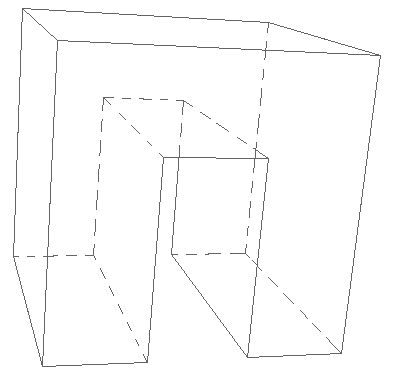
\includegraphics[clip,width=80mm]{Pi.png}          
}		
	\caption{Pi-cube}
	\label{Pi-cube}
\noindent\centering{
    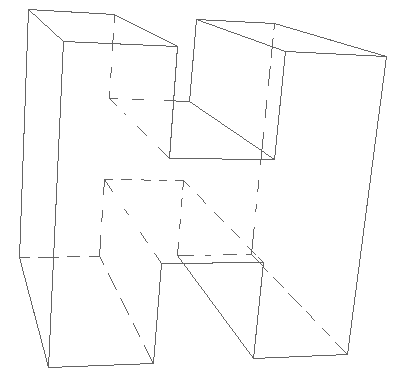
\includegraphics[clip,width=80mm]{H.png}
}		
	\caption{H-cube}
	\label{H-cube}
\end{multicols}
\end{figure}

Тензоры инерции могут сказать нам о несовпадении многогранников, как площади их поверхностей и объемы. Причем это три разных 
характеристики. На  Рис.\ref{Pi-cube} и Рис.\ref{H-cube} изображены два куба с  ребром 6, из которых вырезали части так,
чтобы они стали похожи на буквы $\Pi$ и $\rm H$ соответственно. Посчитаем для них описанными алгоритмами  объем, площадь,
тензор и оси инерции и матричную норму матрицы разности тензоров. Будем использовать $\|A\| = \max\limits_i \sum\limits_j |a_{ij}|$. 
 
 

Вывод программы:

Pi-cube
volume = 168.000000, area = 248.000000
\[
J = 
\begin{Vmatrix}
1167.9999999999997	& 0.0000000000000000 &	-0.000000000000020	\\
0.0000000000000000	& 1039.9999999999993 &   0.0000000000000151	\\
-0.000000000000020	& 0.0000000000000151 &   1136.0000000000002	
\end{Vmatrix}
\]
l0 = 1168.000000, l1 = 1040.000000, l2 = 1136.000000\\
v0 = ( 1.000000,  0.000000, -0.000000)\\
v1 = (-0.000000,  1.000000, -0.000000)\\
v2 = ( 0.000000,  0.000000,  1.000000)\\


H-cube 
volume = 168.000000, area = 248.000000
\[
J = 
\begin{Vmatrix}
	1072.00000000000000	& -0.000000000000003 & -0.000000000000003	\\
	-0.0000000000000037	& 943.99999999999965 & 0.0000000000000289	\\
	-0.0000000000000036	& 0.0000000000000289 & 1136.0000000000002	
\end{Vmatrix}
\]
l0 = 1072.000000, l1 = 944.000000, l2 = 1136.000000\\
v0 = (1.000000, -0.000000, 0.000000)\\
v1 = (0.000000, 1.000000, -0.000000)\\
v2 = (-0.000000, 0.000000, 1.000000)\\

norm = 96.000000\\

Видно, что у многогранников совпадают площади поверхностей и объемы. У многогранников различные моменты инерции относительно 
осей $Ox$ и $Oy$. Совпадают  моменты инерции относительно оси $Oz$. Матричная норма матрицы разности тензоров довольно велика.
О различии двух данных многогранников нельзя сказать оперируя только данными о величинах  их объемов и площадях поверхностей,
но благодаря тензору инерции мы можем их отличить. 

Вычисляя объемы и площади семи тестовых многогранников мы начали подозревать, что последние три многогранника могут быть очень похожи. Найдем их тензоры инерции и попарно нормы матриц разности тензоров. \\
\newpage

Вывод программы:

2009 08 17 brilliant 1.27ct lexus 400c Wol 1
\[
J = 
\begin{Vmatrix}
1781.4231287948823592 &	-0.6909889375148013	& 16.1227320336066455	\\
-0.6909889375148013	& 1782.2249275949866387 & 	-19.6304480276357758	\\
16.1227320336066455	& -19.6304480276357758 & 	302.8415232666940256	\\
\end{Vmatrix}
\]

2009 08 17 brilliant 1.27ct lexus 400c wol 2
\[
J = 
\begin{Vmatrix}
	1781.4003594438154323 &	-0.6910002430205394 &	16.1186652033582227	\\
	-0.6910002430205394	 & 1782.2011283071838079	& -19.6436391040088196\\
	16.1186652033582227	& -19.6436391040088196	& 302.8374053805309245	\\
\end{Vmatrix}
\]

2009 08 17 brilliant 1.27ct lexus 400c wol 3
\[
J = 
\begin{Vmatrix}
1781.2055442779455916 &	-0.6911546540330920 &	16.1192528583386583	\\
-0.6911546540330920 &	1782.0125895182204658 &	-19.6278493699398595	\\
16.1192528583386583 &	-19.6278493699398595 &	302.7826775996047104	\\
\end{Vmatrix}
\]

norm12 =  0.022769\\

norm13 =  0.217585\\

norm23 =  0.194815\\



\newpage
\section{Совмещение двух контуров}
 Описанными выше методами мы научились ставить многогранники в стандартное положение, но у нас довольно мало 
информации о том, как сравнивать два многогранника, находящихся в таком положении. Для того, чтобы сравнить 
два многогранника, предварительно проведем коррекцию, т.е. повороты на малые углы контуров, полученных проецированием 
многогранника на координатные плоскости. Вместе с контурами повернем многогранники им соответствующие.

\subsection{Постановка задачи}
Рассмотрим следующую задачу. Даны два отцентрированных контура. Предположительно они эквивалентны с точностью до  поворота на 
угол $\alpha$ вокруг центра. Задача заключается в том, чтобы найти этот угол. Дополнением к 
поставленной задаче является  поиск некоторой нормы, которая говорила бы нам о том, в какой степени различаются рассматриваемые 
контуры.

\subsection{Начальный этап решения задачи}
\subsubsection{Переход в полярную систему координат}

\begin{figure}[h]
\noindent\centering{
    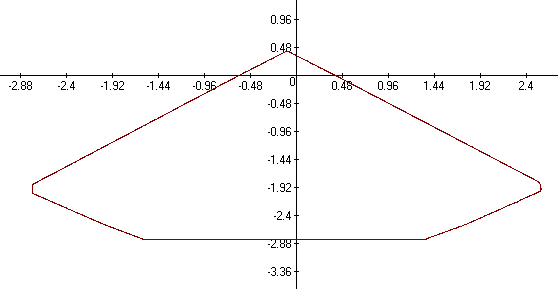
\includegraphics[clip,width=100mm]{4k-contur-1.png}
          }
\caption{Теневой контур}
\label{4k-contur-1}
\end{figure}

\begin{figure}[h]
\noindent\centering{
    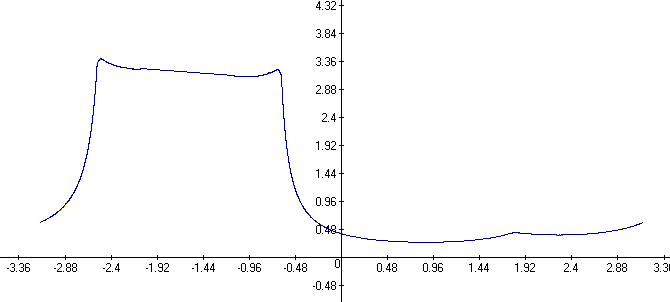
\includegraphics[clip,width=100mm]{4k-contur-per.png}
          }
\caption{Теневой контур в полярной системе координат}
\label{4k-contur-per}
\end{figure}


Контур задан набором координат в декартовой системе $(x,y)$ (см. Рис. \ref{4k-contur-1}). Декартовы координаты $(x,y)$ могут быть 
преобразованы в полярные координаты $(\varphi,\rho)$. Используя тригонометрические функции синус и косинус, преобразуем 
координаты 
в полярные. Будем считать, что  $\varphi\in (-\pi;\pi]$, тогда достаточно воспользоваться следующими формулами:
$$\rho = \sqrt{ {x}^{2} + {y}^{2} }$$

\[
\varphi = 
 	\left\{
 		\begin{aligned}
  		& arctan\left(\frac{x}{y}\right),       & \text{если}\;x>0 & \\
 		& arctan\left(\frac{x}{y}\right) + \pi, & \text{если}\;x<0 &\;\text{и}\;y\ge 0\\
  		& arctan\left(\frac{x}{y}\right) - \pi, & \text{если}\;x<0 &\;\text{и}\;y<0 \\
  		& \mspace{70mu}\frac{\pi}{2},                        & \text{если}\;x=0 &\;\text{и}\;y>0 \\
  		& \mspace{48mu}-\frac{\pi}{2},    					& \text{если}\;x=0 &\;\text{и}\;y<0 \\
		& \mspace{72mu}    	0,								& \text{если}\;x=0 &\;\text{и}\;y=0 \\
		\end{aligned}
	\right.
\]

Теперь заметим, что каждому контуру стала соответствовать $2\pi$-периодическая функция 
$\rho = \rho(\varphi)$ (см. Рис. \ref{4k-contur-per}).

\subsubsection{Интерполяция на равномерную сетку}
Можно проводить различные операции с данными функциями, в том числе и интегрировать. Для того  чтобы проинтегрировать данные 
функции, проведём их интерполяцию на равномерную сетку.  В декартовой системе координат прямую можно задать уравнением
 $Ax+By+C=0$. 

Соответствующую ей прямую в полярных координатах можно задать уравнением $A\rho\cos\varphi+B\rho\sin\varphi+C=0$. Соединим все 
точки контура прямыми и получим  ломанную кривую. Можно считать, что ни одна прямая не проходит через начало координат.  Положим 
для удобства коэффициент $C=-1$. Тогда по двум точкам $({\varphi}_{1}, {\rho}_{1})$ и $({\varphi}_{2}, {\rho}_{2})$  можно 
вычислить коэффициенты прямой через них проходящей из следующей системы:

\[
\varphi = 
 	\left\{
 		\begin{aligned}
  		A{\rho}_{1}\cos{\varphi}_{1}+B{\rho}_{1}\sin{\varphi}_{1}-1=0 \\
 		A{\rho}_{2}\cos{\varphi}_{2}+B{\rho}_{2}\sin{\varphi}_{2}-1=0 \\
		\end{aligned}
	\right.
\]

Затем найдем коэффициенты прямой:
\begin{center}
$A = 
\frac
{{\rm det} \begin{pmatrix} 1 & {\rho}_{1}\sin{\varphi}_{1} \\ 1 & {\rho}_{2}\sin{\varphi}_{2} \end{pmatrix} }
{{\rm det} \begin{pmatrix} {\rho}_{1}\cos{\varphi}_{1} & {\rho}_{1}\sin{\varphi}_{1} \\ {\rho}_{2}\cos{\varphi}_{2} & {\rho}_{2}\sin{\varphi}_{2} \end{pmatrix} }
$
$B = 
\frac
{{\rm det} \begin{pmatrix}  {\rho}_{1}\cos{\varphi}_{1}  & 1\\  {\rho}_{2}\cos{\varphi}_{2} & 1\end{pmatrix} }
{{\rm det} \begin{pmatrix} {\rho}_{1}\cos{\varphi}_{1} & {\rho}_{1}\sin{\varphi}_{1} \\ {\rho}_{2}\cos{\varphi}_{2} & {\rho}_{2}\sin{\varphi}_{2} \end{pmatrix} }
$
\end{center}

Зная, какой прямой соединены точки, можно брать точки с этой прямой с каким-то заданным шагом ${\varphi}_{0}$.  Это и будет наша 
интерполяция на равномерную сетку. Полученная интерполяция дает разбиение отрезка $[-\pi;\pi]$. Теперь мы можем проинтегрировать 
функцию, соответствующую контуру методом трапеций.

$$I = \frac{1}{2}\sum_{i=1}^{n}({\varphi}_{i}-{\varphi}_{i-1})({\rho}_{i}-{\rho}_{i-1})$$

Этот навык необходим в данной задаче, потому что далее мы будем раскладывать периодические функции в ряд Фурье и работать уже с 
полученными рядами.

\subsubsection{Разложение периодических функций в ряды Фурье}
Тригонометрическим рядом Фурье функции $f\in{\rm L}_{2}[-\pi;\pi]$ называют функциональный ряд вида:
$$f(x)= \frac{{a}_{0}}{2} + \sum\limits_{n=1}^{\infty} ({a}_{n}cos(nx)+{b}_{n}sin(nx)),$$     где
${a}_{0}= \frac{1}{\pi} \int\limits_{-\pi}^{\pi}f(x)dx,$
${a}_{n} = \frac{1}{\pi} \int\limits_{-\pi}^{\pi}f(x)\cos(nx)dx,$
${b}_{n} = \frac{1}{\pi} \int\limits_{-\pi}^{\pi}f(x)\sin(nx)dx.$

Ряд  Фурье сходиться к функции $f$ в пространстве   ${\rm L}_{2}[-\pi;\pi]$. Иными словами, если обозначить  через  ${S}^{k}(x)$ частичные суммы ряда, то их среднеквадратичное  отклонение от функции $f$ стремиться к нулю.
$${S}^{k}(x) = \frac{{a}_{0}}{2} + \sum\limits_{n=1}^{k} ({a}_{n}cos(nx)+{b}_{n}sin(nx))$$
$$\lim_{k \to \infty} \int\limits_{-\pi}^{\pi}(f(x)-S^{k}(x))^{2}dx = 0$$

Мы ищем угол поворота одного контура относительно другого, т.е.  для $2\pi$-периодических 
функций $f_{1}(x)$ и $f_{2}(x)$ существует такой угол $\alpha$, что $f_{1}(x) = f_{2}(x + \alpha) $. 
Функциям $f_{1}(x)$ и $f_{2}(x)$  соответствуют частичные суммы их рядов Фурье $S_{1}(x)$ и $S_{2}(x)$. 
Введем функцию  $\Phi(\alpha)  = \| f_{1}(x) - f_{2}(x + \alpha)\|^{2}$ и распишем её в соответствии с определением.

\[
 	\left.
 		\begin{aligned}
  		{f}_{1}(\varphi) &=& \frac{{a}^{'}_{0}}{2} + \sum\limits_{n=1}^{\infty} ({a}^{'}_{n}\cos(n\varphi)+{b}^{'}_{n}\sin(n\varphi)) \\
 		{f}_{2}(\varphi + \alpha) &=& \frac{{a}^{''}_{0}}{2} + \sum\limits_{n=1}^{\infty} ({a}^{''}_{n}\cos(n\varphi+ \alpha)+{b}^{''}_{n}\sin(n\varphi+ \alpha)) \\
		\end{aligned}
	\right\rbrace	
	\Rightarrow
\]
$$\Biggl \|\frac{{a}^{'}_{0}}{2} + \sum\limits_{n=1}^{\infty} ({a}^{'}_{n}\cos(n\varphi)+{b}^{'}_{n}\sin(n\varphi)) - 
\frac{{a}^{''}_{0}}{2} + \sum\limits_{n=1}^{\infty} ({a}^{''}_{n}\cos(n\varphi+ \alpha)+{b}^{''}_{n}\sin(n\varphi+ \alpha)) \Biggr \|^{2} 
=$$
$$
\Biggl \|
\sum\limits_{n=1}^{\infty} {a}^{'}_{n}\cos(n\varphi)+ \sum\limits_{n=1}^{\infty}{b}^{'}_{n}\sin(n\varphi) - 
\sum\limits_{n=1}^{\infty} {a}^{''}_{n}\cos(n\varphi+ \alpha)+ \sum\limits_{n=1}^{\infty}{b}^{''}_{n}\sin(n\varphi+ \alpha) 
\Biggr \|^{2}
=$$
$$
\Biggl \|
\sum\limits_{n=1}^{\infty} ({a}^{'}_{n} - {a}^{''}_{n}\cos(n\alpha) - {b}^{''}_{n}\sin(n\alpha)) + 
\sum\limits_{n=1}^{\infty} ({b}^{'}_{n} - {a}^{''}_{n}\sin(n\alpha) - {b}^{''}_{n}\sin(n\alpha)) 
\Biggr \|^{2}
=$$
$$
\sum\limits_{n=1}^{\infty} ({a}^{'}_{n} - {a}^{''}_{n}\cos(n\alpha) - {b}^{''}_{n}\sin(n\alpha))^{2} + 
\sum\limits_{n=1}^{\infty} ({b}^{'}_{n} - {a}^{''}_{n}\sin(n\alpha) - {b}^{''}_{n}\sin(n\alpha))^{2} 
$$

Функция $\Phi(\alpha)$ будет той самой нормой, о которой говорилось вначале. Это наш показатель различия двух контуров. Теперь 
нужно найти такой угол $\alpha$, при котором значение функции $\Phi(\alpha)$ минимально. Такой угол $\alpha$ будет искомым.

\subsubsection{Пример приближения функции частичной суммой ряда Фурье}
\begin{figure}[h]
\noindent\centering{
    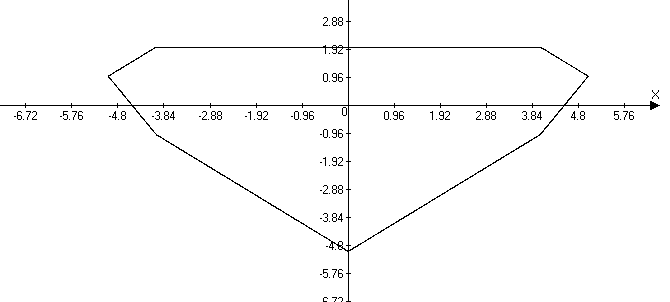
\includegraphics[clip,width=100mm]{4k-contur-fur.png}
          }
\caption{Контур приближенный частичной суммой ряда Фурье}
\label{4k-contur-fur}
\end{figure}

По теореме  Карлесона\cite{kolm}  если $f \in {\rm L}_{2}[-\pi;\pi]$(как в нашем случае), 
то её ряд Фурье сходится к ней почти всюду.  
Наглядно  работу с рядами можно продемонстрировать, если для  простого контура, составленного всего по двенадцати точкам, 
провести все описанные выше действия (см. Рис. \ref{4k-contur-fur}).  

\begin{figure}[h]
\noindent\centering{
    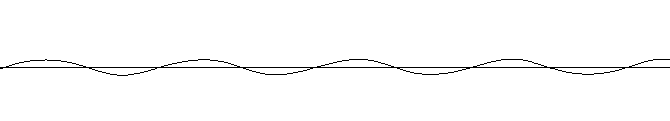
\includegraphics[clip,width=150mm]{4k-contur-fsmol.png}
          }
\caption{Увеличенный участок контура}
\label{4k-contur-fsmol}
\end{figure}

Контур, изображенный на Рис. \ref{4k-contur-fur}, состоит из прямых. При увеличении изображения можно увидеть каким образом функция частичной суммы $S^{1000}(x)$ приближает исходную функцию $f(x)$. Функция ${S}^{k}(x)$ будет «обвивать» функцию 
$f(x)$ (см. Рис. \ref{4k-contur-fsmol}).

\subsection{Поиск оптимального угла поворота}
\subsubsection{Область поиска угла}
После того, как мы нашли коэффициенты рядов Фурье каждого контура, займемся поиском угла, при котором значение функции  
$\Phi(\alpha)$ минимально.  В идеале $\Phi(\alpha) = 0$.  Заметим, что $\Phi(\alpha)$ -- это тоже ряд Фурье, и равенство его нулю 
говорит о равенстве нулю его коэффициентов. 

Пользуясь сходимостью рядов Фурье, мы используем частичные суммы ряда и вычисляем конечное число коэффициентов. Фактически мы 
пользуемся функцией $\Phi_{k}(\alpha) = \|{S}_{1}(\varphi) - {S}_{2}(\varphi + \alpha) \|^{2}$.  Коэффициенты данного ряда 
образуют $\rm N$ систем из двух уравнений.
\[ 
 	\left\{
 		\begin{aligned}
  		{a}^{'}_{n} - {a}^{''}_{n}\cos(n\alpha) - {b}^{''}_{n}\sin(n\alpha) = 0\\
 		{b}^{'}_{n} - {a}^{''}_{n}\sin(n\alpha) - {b}^{''}_{n}\sin(n\alpha) = 0\\
		\end{aligned}
	\right.
	\text{, где}\;n = {\rm 1...N}
\]

Решая эти системы, мы находим $\rm N$ углов ${\alpha}_{1}...{\alpha}_{\rm N}$. Они довольно кучно расположены в окрестности 
предполагаемого угла поворота. На Рис. \ref{4k-alpha} можно посмотреть расположение улов ${\alpha}_{k}$ для контуров, которые внешне выглядят, как контур на Рис. \ref{4k-contur-1}. Эти углы принадлежат отрезку $[ {\alpha}_{min};{\alpha}_{max} ]$ 
которому, предположительно, принадлежит и наш угол.
\begin{figure}[h]
\noindent\centering{
    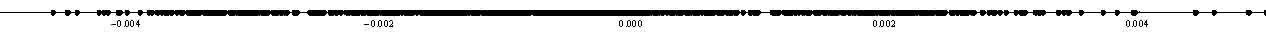
\includegraphics[clip,width=150mm]{4k-alpha.png}
          }
\caption{Расположение углов на оси $\alpha$}
\label{4k-alpha}
\end{figure}

\subsubsection{Поиск оптимального угла разложением до первого порядка}
При нахождении минимума функции $\Phi_{k}(\alpha)$ хотелось  бы обойтись как можно меньшим числом операций. Это наводит на мысль 
воспользоваться разложением слагаемых $\Phi_{k}(\alpha)$ в ряд Тейлора до первого порядка в точке ${\alpha}_{0}$. Тогда мы получим 
функцию $\Phi_{k}^{1}(\alpha)$, которая будет квадратичной, и её минимум будет достигаться в вершине.  Для найденной вершины 
разложение и поиск экстремума можно  будет повторить. 

Подробнее рассмотрим эту идею. Синусы и косинусы мы заменим на их линейные приближения. Коэффициенты линейной функции, полученные 
из тригонометрических функций, взятых точке $n{\alpha}_{0}$ обозначим  $A^{n}_{1}$, $B^{n}_{1}$,  $A^{n}_{1}$ и $B^{n}_{2}$.
\[ 
 		\begin{aligned}
  		\cos(n\alpha) = -n\sin(n\alpha_{0})\alpha + (\cos(n\alpha_{0}) + n\alpha_{0}\sin(n\alpha_{0})) = A^{n}_{1}\alpha + B^{n}_{1}\\
 		\sin(n\alpha) = -n\cos(n\alpha_{0})\alpha + (\sin(n\alpha_{0}) + n\alpha_{0}\cos(n\alpha_{0})) = A^{n}_{2}\alpha + B^{n}_{2}\\
		\end{aligned}
\]

В явном виде $\Phi_{k}^{1}(\alpha)$ нам не понадобиться, пользоваться мы будем её производной, от которой будем брать корень, как 
последующую точку разложения. Обозначим эту производную, как $D_{k}^{1}(\alpha)$.

$$
D_{k}^{1}(\alpha) = \sum \limits_{n=1}^{N} 
	\Biggl(
		2(A^{n}_{1}a^{''}_{n} + A^{n}_{2}b^{''}_{n}) 
			\Bigl( 
				-a^{'}_{n} + a^{''}_{n}(B^{n}_{1} + A^{n}_{1}\alpha) + b^{''}_{n}(B^{n}_{2} + A^{n}_{2}\alpha)
			\Bigr) 
	\Biggr) +
$$

$$
+ \sum \limits_{n=1}^{N}
	\Biggl(
		2(a^{'}_{n}A^{n}_{2} - A^{n}_{1}b^{''}_{n})
			(b^{'}_{n} - B^{n}_{1}b^{''}_{n} + a^{'}_{n}B^{n}_{2} + a^{'}_{n}A^{n}_{2}\alpha - A^{n}_{1}b^{''}_{n}\alpha)
	\Biggr)
$$

Этот алгоритм оправдывает себя скоростью и однозначностью результата. После нескольких итераций ответ получается таким же, каким 
бы он был, если бы мы взяли какой-то другой угол из нашего отрезка. В этом есть плюсы и минусы. Явный плюс это стабильность и 
однозначность. Но однозначность порой портит результат. В этом и есть минус алгоритма. Рассмотрим такую ситуацию. Мы взяли какой-
то угол, который оказался очень близок к  оптимальному углу (оптимальный угол обозначим $\alpha_{opt}$). Проделали несколько 
итераций и получили ответ. Все бы хорошо, но ответ получился хуже, чем начальный угол. Это происходит собственно из-за того, что 
мы пользуемся только первым порядком при разложении.

\subsubsection{Метод золотого сечения}
Метод золотого сечения -- это метод поиска значений  функции на заданном отрезке. В нашем случае это 
отрезок  $[ {\alpha}_{min};{\alpha}_{max} ]$
(та самая область поиска угла). В основе метода лежит принцип деления в пропорциях золотого сечения. Наиболее широко метод 
золотого сечения известен, как метод поиска экстремума в решении задач оптимизации. Этот метод схож с троичным поиском, когда 
отрезок делят на три 
части. Но в нашем случае он будет более эффективен  и полезен, т.к. за одну итерацию вычисление функции занимает больше всего 
времени.

Опишем алгоритм формально для поиска минимума функции $f(x)$. 
Пропорцию золотого сечения обозначим $\phi = \frac{1+\sqrt{5}}{2}$. 
Пусть заданы начальные границы $a$ и $b$ отрезка  и точность $\varepsilon$.\\
{\bf A}: Найдем начальные точки деления и значения функции в них.
\begin{center} 
${x}_{1} = b - \frac{b-a}{\phi}$\qquad                
${x}_{2} = a + \frac{b-a}{\phi}$\qquad
${y}_{1} = f({x}_{1})$\qquad
${y}_{2} = f({x}_{2})$
\end{center}
{\bf B}:	  

{\bf   если $\bf {y}_{1} \le {y}_{2}$}
\begin{center} 
$b = {x}_{2}$\qquad                
${x}_{2} = {x}_{1}$\qquad
${x}_{1} = b - \frac{b-a}{\phi}$\qquad
${y}_{2} = {y}_{1}$\qquad
${y}_{1} = f({x}_{1})$
\end{center}

{\bf иначе}
\begin{center} 
$a = {x}_{1}$\qquad                
${x}_{1} = {x}_{2}$\qquad
${x}_{2} = a + \frac{b-a}{\phi}$\qquad
${y}_{1} = {y}_{2}$\qquad
${y}_{2} = f({x}_{2})$
\end{center}
{\bf C}:	  

{\bf   если $\bf |b - a| < \varepsilon$}
\begin{center} 
${x} = \frac{a + b}{2}$
{\bf конец алгоритма}
\end{center}

{\bf   иначе}
\qquad{\bf переход к B}

\subsubsection{Промежуточное тестирование}
Ниже будут размещены результаты работы двух алгоритмов. Было проведено 200
тестов. Каждый раз рассматривалось два контура подобных тем, что были изображены на Рис. \ref{4k-contur-1}.

\begin{center}
\footnotesize
\begin{longtable}{|p{0.5cm}|p{3.5cm}|p{3.5cm}|p{3.5cm}|p{3.5cm}|}
\hline
№ & угол ${\alpha}_{1}$, найденный методом \;\;\; золотого сечения & Значение функции $\Phi_{1000}(\alpha_{1})$  
& угол ${\alpha}_{2}$, найденный  методом разложения до первого порядка
& Значение функции $\Phi_{1000}(\alpha_{2})$  \endhead
\hline
1  & 0.0000000006187237  & 0.0000364903138242  & -0.0001246371718166  & 1.7671189009773765\\
\hline
2  & -0.0000000002130303  & 0.0000241248027327  & -0.0001780904338699  & 3.6086038252644590\\
\hline
3  & 0.0000000004096531  & 0.0000330686559986  & 0.0000666720871369  & 0.5100554328342735\\
\hline
4  & 0.0070366143405668  & 160.5602609387167100  & -0.0000813677608900  & 0.7610093193291561\\
\hline
5  & 0.0000000006909003  & 0.0000441342332882  & -0.0001061538794230  & 1.2948973975183360\\
\hline
\dots  & \dots  		 & \dots  			   & \dots  			  & \dots \\
\hline
196  & -0.0000000000294111  & 0.0000228051225801  & -0.0000143841768123  & 0.0233150592256847\\
\hline
197  & -0.0000000008048337  & 0.0000206697409735  & -0.0000672396357149  & 0.5090763949550948\\
\hline
198  & -0.0038645586592030  & 147.7111390403078400  & -0.0000150250519554  & 0.0254951321585966\\
\hline
199  & 0.0000000001651253  & 0.0000084653900745  & -0.0000927534629075  & 0.9711278852750874\\
\hline
200  & -0.0000000000854542  & 0.0000143060688675  & -0.0000577173517984  & 0.3774375762069376\\
\hline
\caption{Результаты отдельной работы алгоритмов}
\label{4k-tab-1-sm}
\end{longtable}
\end{center}

По этим данным видно, что метод золотого сечения не всегда дает достаточно точный результат, но чаще случаи, когда угол, 
полученный этим методом, на порядок точнее угла, полученного методом разложения до первого порядка. В чём же причина «осечек» 
метода золотого сечения? 

Рассмотрим функцию $\Phi_{k}(\alpha)$. Она обладает очень высоким абсолютным значением производной.  
Она очень быстро убывает к нулю, а потом 
так же быстро от нуля и растет.  При этом она подобно примеру, изображенному на Рисунке 6, обвивает функцию, похожую на 
квадратичную.  Это и не удивительно т.к. уже был сделан вывод о том, что $\Phi(\alpha)$ -- это ряд Фурье. Это и мешает методу 
золотого сечения. 
Алгоритм попадает в локальный минимум, которых может быть несколько у функции в области поиска, и там и остается, не доходя до 
глобального минимума.  Когда мы переходим к функции $\Phi_{k}^{1}(\alpha)$ и используем другой алгоритм, локальные минимумы 
пропадают вместе с 
тригонометрическими функциями. Однако так же пропадает и точность.
\subsubsection{Совместная работа алгоритмов}
Само собой напрашивается следующая идея. Стоит скомбинировать два алгоритма. Каким образом это можно сделать? Заметим, что 
алгоритмом, где используется разложение в ряд Тейлора, мы   получаем угол, довольно близкий к оптимальному углу. Далее мы можем 
уже применить метод золотого сечения, но не в области поиска, а в окрестности этого угла. Таким образом, происходит сокращение 
итераций метода золотого сечения, за счет сужения области поиска. И происходит увеличение точности полученного результата.

Ниже  будут размещены  результаты совместной работы  двух алгоритмов. Было также  проведено 200 тестов. Каждый раз 
рассматривалось два контура подобных контуру, изображенном на Рис. \ref{4k-contur-1}.

\begin{center}
\footnotesize
\begin{longtable}{|p{0.5cm}|p{3.5cm}|p{3.5cm}|p{3.5cm}|p{3.5cm}|}
\hline
№ & угол ${\alpha}_{1}$, который является оптимальным & Значение функции $\Phi_{1000}(\alpha_{1})$  
& угол ${\alpha}_{2}$, использующийся для сужения области поиска
& Значение функции $\Phi_{1000}(\alpha_{2})$  \endhead
\hline
1  & 0.0000000006187341  & 0.0000364903138242  & -0.0001246371718166  & 1.7671189009773765\\
\hline
2  & -0.0000000002130293  & 0.0000241248027327  & -0.0001780904338699  & 3.6086038252644590\\
\hline
3  & 0.0000000004096501  & 0.0000330686559986  & 0.0000666720871369  & 0.5100554328342735\\
\hline
4  & -0.0000000000805675  & 0.0000081882589490  & -0.0000813677608900  & 0.7610093193291561\\
\hline
5  & 0.0000000006909011  & 0.0000441342332882  & -0.0001061538794230  & 1.2948973975183360\\
\hline
\dots  & \dots  		 & \dots  			   & \dots  			  & \dots \\
\hline
196  & -0.0000000000294107  & 0.0000228051225801  & -0.0000143841768123  & 0.0233150592256847\\
\hline
197  & -0.0000000008048175  & 0.0000206697409735  & -0.0000672396357149  & 0.5090763949550948\\
\hline
198  & 0.0000000005617723  & 0.0000150056528980  & -0.0000150250519554  & 0.0254951321585966\\
\hline
199  & 0.0000000001651309  & 0.0000084653900745  & -0.0000927534629075  & 0.9711278852750874\\
\hline
200  & -0.0000000000854444  & 0.0000143060688675  & -0.0000577173517984  & 0.3774375762069376\\
\hline
\caption{Результаты совместной работы алгоритмов}
\label{4k-tab-2-sm}
\end{longtable}
\end{center}

Спроецируем на координатные плоскости сравниваемые многогранники и проведем для полученных теневых контуров коррекцию. 
Коррекция проводится, чтобы убедиться, что многогранники сильно совмещены в 
своем стандартном положении. Заметим, если функция $\Phi(\alpha)$ принимает большое значение, тела не совпадают, несмотря
на совпадение остальных характеристик. 


\newpage
\section{Кластеризация}
Два многогранника в одной системе координат находятся в стандартном положении, наша задача ответить на сколько 
сильно они похожи друг на друга.

Для ответа на этот вопрос нам придется воспользоваться методами кластерного анализа. Кластеризация ---
разбиение исходного множества на 
подмножества называемые кластерами, так, чтобы каждый кластер состоял из схожих объектов, 
а объекты разных кластеров существенно отличались. 

Таким отличием, например, может быть расстояние до других 
элементов множества или до каких-то фиктивных элементов, начальному множеству не принадлежащих. 
Для элементов из одного кластера это расстояние маленькое, для элементов из разных 
кластеров, оно большое. Маленькое расстояние или большое мы определяем с помощью порога. Если расстояние между элементами 
больше порога, то считаем, что они лежат в разных кластерах \cite{mand}. 

На многограннике могут присутствовать 
множества граней, которые находятся рядом, причем угол между нормалями к этим граням очень маленький. Бывает ситуация, 
когда при составлении трехмерной модели многогранника, одна грань его представляется в виде нескольких, находящихся в одной 
плоскости. Но даже если таких ситуаций не возникает, имеет смысл провести кластеризацию, чтобы потом сравнить многогранники по 
этим сформировавшимся группам. 
При таком сравнении мы можем выделить участки (кластеры), на которых отличие явно и кластеры на которых наблюдается полное или
частичное сходство.  И сравнивать многогранники можно уже не полностью, а по кластерам \cite{prep}.

Кластеризацию будем проводить считая, что векторы нормали -- это точки на единичной сфере, вес каждой точки -- это площадь 
соответствующей ей грани.
Прежде чем начать описание проведенной кластеризации хотелось бы сказать о теоремах Минковского\cite{mink} :

\newtheorem{Th}{Теорема}
\begin{Th}[Теорема единственности Минковского]\label{thMin1}
Если между гранями двух замкнутых выпуклых многогранников установлено взаимно-однозначное соответствие так, что
\begin{enumerate}
\item единичные нормали к соответствующим граням совпадают
\item площади соответствующих граней одинаковы
\end{enumerate}
то многогранники получаются один из другого параллельным переносом (и, в частности, они конгруэнтны).
\end{Th}

\begin{Th}[Теорема существования Минковского]\label{thMin2}
Если  $\vec n_1, ..., \vec n_k$ —  произвольные единичные векторы, не все направленные в одно полупространство, 
и $S_1, ..., S_k$  — произвольные положительные числа, причём $\vec n_1 S_1 + ...+\vec n_k S_k = 0$, то существует выпуклый 
многогранник, для которого векторы
$\vec n_1, ...,\vec n_k$  (и только они) являются векторами внешних единичных нормалей к граням, а числа  
$S_1, ..., S_k$ являются площадями граней.
\end{Th}

Это теоремы о существовании и единственности замкнутого выпуклого многогранника с заданными направлениями нормалей
и площадями граней. Из них мы можем сделать следующие выводы о предстоящей кластеризации:
\begin{enumerate} 
\item проведя кластеризацию, мы сопоставим исходному многограннику
какой-то другой с меньшим числом граней и возможно другим направлением нормалей. 
\item с помощью теоремы единственности мы можем установить конгуэнтность двух многогранников, если задано, указанное в теореме,
взаимно-однозначное соответствие.
\end{enumerate}

Таким образом, мы можем применить одну и ту же кластеризацию для двух многогранников, и посмотреть есть ли соответствие между
полученными кластерами. Если такое соответствие найдется, то можно говорить о схожести рассмотренных многогранников. 

\subsection{Иерархический алгоритм кластеризации}
Многогранник представляет собой набор граней с известной площадью и известными векторами нормали единичной длины. Векторы 
нормали представляют собой точки на единичной сфере. У каждой такой точки есть вес. Вес точки на сфере -- это величина площади 
грани, ей соответствующей. 

Проведем кластеризацию следующим образом. 

Кластером будем считать структуру, состоящую из списка граней, 
центра кластера, и веса кластера. Центр кластера иногда называют главной точкой кластера. 
Расстояние между кластерами -- это расстояние между их главными точками на единичной сфере.  

Изначально каждую точку на единичной сфере, соответствующую грани многогранника, будем считать кластером. Главной точкой такого
кластера является нормаль к грани, вес кластера -- это площадь грани, список граней содержит только одну грань.   

Найдем два ближайших кластера и объединим их в один \cite{hier}. Новый кластер включает в себя все грани, которые содержали 
кластеры его образовавшие. Вес нового кластера -- это сумма весов образовавших его кластеров. Центр вычисляется, как
сумма, состоящая из центров, составляющих кластер граней, умноженных на их вес, поделенная на вес всего кластера.
Центр считается таким образом для того, чтобы он смещался тем сильнее или слабее, чем больше или меньше кластер,
с которым происходит слияние. 

После объединения двух ближайших кластеров мы получили новый набор кластеров, число которых на единицу меньше. 
За конечное число шагов мы придем к ситуации, что все кластеры сольются в один. Но можно прекратить это слияние и раньше,
например, когда ближайшее расстояние между кластерами будет больше заранее определенной величины (порога кластеризации).

В следующем разделе показано, как происходит слияние кластеров, описанным алгоритмом, на примере многогранника, 
изображенном на Рис.\ref{1201821}-\ref{510611}.
\subsection{Пример иерархической кластеризации}
\begin{figure}[h]
\noindent
\begin{multicols}{2}
\noindent\centering{
    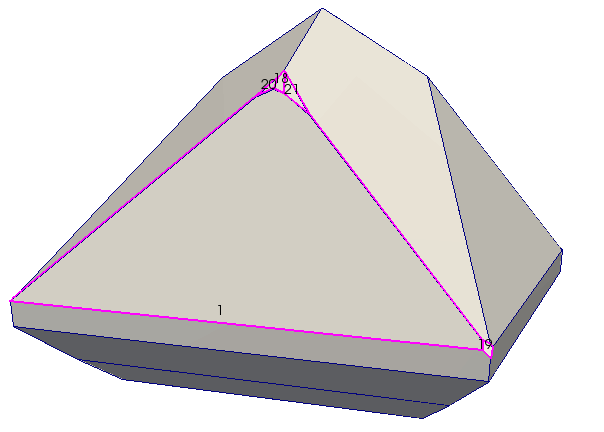
\includegraphics[clip,width=85mm]{poly-small1201821.png}          
}		
	\caption{Объединение граней 1, 19, 20, 18, 21  в кластер}
	\label{1201821}
\noindent\centering{
    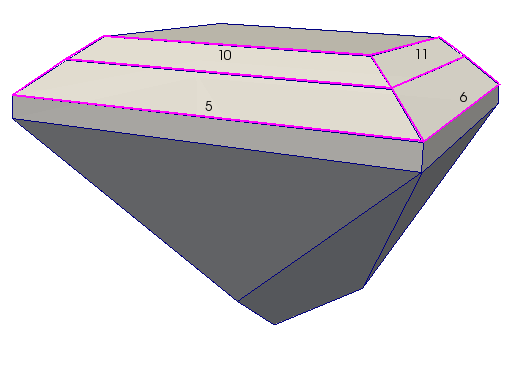
\includegraphics[clip,width=85mm]{poly-small510611.png}
}		
	\caption{Пример очень близких граней многогранника}
	\label{510611}
\end{multicols}
\end{figure}
Данный многогранник представляет собой многогранник, состоящий из 48 ребер и 26 вершин. На нем наблюдаются сколы. Один 
из таких сколов представлен гранями с номерами 18, 20 и 21. Иерархическим алгоритмом на шестом шаге мы получаем 
слияние граней 1, 18, 19, 20 и 21 (см. Рис.\ref{1201821} ). На первых шагах мы наблюдаем слияние очень близких граней(6 и 11, 5 и 10 и т.д.), они  выделены на Рис.\ref{510611}

В один кластер на самом деле могут попасть грани, лежащие довольно далеко друг от друга. Еще одной проблемой для решения 
задачи сравнения многогранников является то, что кластеризация на определенном шаге зависит от начальной кластеризации 
многогранника. Например, у нас есть две модели  ограненного бриллианта. У них один вес и одна и та же огранка.
Но при этом мы получили разные модели за счет того, что в рундисте присутствует очень большое число граней. Та же ситуация может 
произойти при составлении трехмерной модели одного камня с разной точностью. Получив две разные кластеризации одного и 
того же камня, мы можем прийти к выводу, что это модели двух разных камней, что недопустимо при решении задачи сравнения 
многогранников.  

Ниже представлен вывод программы в которой реализован описанный алгоритм. В фигурных скобках список граней и вес кластера.
Выводится шаг алгоритма, расстояние между сливаемыми кластерами, номера граней, помеченные нулем или единицей в зависимости от 
того была ли грань добавлена в другой кластер.
\newpage
Вывод программы кластеризации многогранника, изображенного на Рис.\ref{1201821}-\ref{510611} :

-----------------------    0    ------------------------\\
id0 = 6, id1 = 11, distance(id0, id1) = 0.041857\\
clusterid0 = \{6, ; area = 4.123551\}, clusterid1 = \{11, ; area = 2.348499\}\\
-----------------------    1    ------------------------\\
id0 = 7, id1 = 8, distance(id0, id1) = 0.044310\\
clusterid0 = \{7, ; area = 3.908858\}, clusterid1 = \{8, ; area = 2.322030\}\\
-----------------------    2    ------------------------\\
id0 = 5, id1 = 10, distance(id0, id1) = 0.045199\\
clusterid0 = \{5, ; area = 4.106649\}, clusterid1 = \{10, ; area = 2.379896\}\\
-----------------------    3    ------------------------\\
id0 = 4, id1 = 9, distance(id0, id1) = 0.046769\\
clusterid0 = \{4, ; area = 3.944632\}, clusterid1 = \{9, ; area = 2.323428\}\\
-----------------------    4    ------------------------\\
id0 = 18, id1 = 21, distance(id0, id1) = 0.066672\\
clusterid0 = \{18, ; area = 0.030149\}, clusterid1 = \{21, ; area = 0.056550\}\\

На первых четырех этапах мы видим объединение очень близких кластеров. Пока в объединяемых кластерах содержится только 
по одной грани. Эти грани практически гладко состыкованы и законно стоят первыми кандидатами на слияние. Порог слияния довольно мал, например следующем этапе порог слияния вырастет почти в четыре раза. 
\\

\noindent
-----------------------    5    ------------------------\\
id0 = 1, id1 = 20, distance(id0, id1) = 0.226213\\
clusterid0 = \{1, ; area = 9.243519\}, clusterid1 = \{20, ; area = 0.021866\}\\
-----------------------    6    ------------------------\\
id0 = 1, id1 = 18, distance(id0, id1) = 0.259093\\
clusterid0 = \{1, 20, ; area = 9.265386\}, clusterid1 = \{18, 21, ; area = 0.086699\}\\
-----------------------    7    ------------------------\\
id0 = 1, id1 = 19, distance(id0, id1) = 0.441366\\
clusterid0 = \{1, 20, 18, 21, ; area = 9.352084\}, clusterid1 = \{19, ; area = 0.012343\}\\
-----------------------    8    ------------------------\\
id0 = 1, id1 = 14, distance(id0, id1) = 0.522099\\
clusterid0 = \{1, 20, 18, 21, 19, ; area = 9.364427\}, clusterid1 = \{14, ; area = 1.913411\}\\

На 5-8 шаге видно слияние большой грани под номером 1 с маленькими гранями, которые образованы в результате сколов.
Грани, которые попали в один кластер выделены на рисунке \ref{1201821}.  
\\

\noindent
\newpage

-----------------------    9    ------------------------\\
id0 = 3, id1 = 16, distance(id0, id1) = 0.536131\\
clusterid0 = \{3, ; area = 9.233654\}, clusterid1 = \{16, ; area = 2.062748\}\\
-----------------------    10    ------------------------\\
id0 = 0, id1 = 17, distance(id0, id1) = 0.540989\\
clusterid0 = \{0, ; area = 9.318728\}, clusterid1 = \{17, ; area = 2.093047\}\\
-----------------------    11    ------------------------\\
id0 = 2, id1 = 15, distance(id0, id1) = 0.558522\\
clusterid0 = \{2, ; area = 9.277046\}, clusterid1 = \{15, ; area = 2.050655\}\\
-----------------------    12    ------------------------\\
id0 = 13, id1 = 24, distance(id0, id1) = 0.705729\\
clusterid0 = \{13, ; area = 0.000312\}, clusterid1 = \{24, ; area = 6.043018\}\\
-----------------------    13    ------------------------\\
id0 = 6, id1 = 12, distance(id0, id1) = 0.727288\\
clusterid0 = \{6, 11, ; area = 6.472050\}, clusterid1 = \{12, ; area = 16.448372\}\\
-----------------------    14    ------------------------\\
id0 = 5, id1 = 6, distance(id0, id1) = 0.599316\\
clusterid0 = \{5, 10, ; area = 6.486545\}, clusterid1 = \{6, 11, 12, ; area = 22.920422\}\\
-----------------------    15    ------------------------\\
id0 = 4, id1 = 5, distance(id0, id1) = 0.603477\\
clusterid0 = \{4, 9, ; area = 6.268060\}, clusterid1 = \{5, 10, 6, 11, 12, ; area = 29.406967\}\\
-----------------------    16    ------------------------\\
id0 = 1, id1 = 23, distance(id0, id1) = 0.746862\\
clusterid0 = \{1, 20, 18, 21, 19, 14, ; area = 11.277839\}, clusterid1 = \{23, ; area = 6.137587\}\\
-----------------------    17    ------------------------\\
id0 = 0, id1 = 22, distance(id0, id1) = 0.752870\\
clusterid0 = \{0, 17, ; area = 11.411775\}, clusterid1 = \{22, ; area = 6.012501\}\\
-----------------------    18    ------------------------\\
id0 = 3, id1 = 25, distance(id0, id1) = 0.762633\\
clusterid0 = \{3, 16, ; area = 11.296402\}, clusterid1 = \{25, ; area = 5.951327\}\\


Далее мы наблюдаем падение порога слияние. Это происходит, по следующей причине.
Последние несколько слияний проходили с довольно большим порогом и многогранник практически полностью оказался разбит на 
весомые кластеры. Теперь происходит слияние этих гигантов (Рис. \ref{32516215}).   

\begin{figure}[h]
\noindent\centering{
    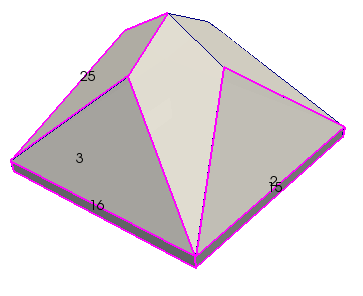
\includegraphics[clip,width=60mm]{32516215.png}
          }
\caption{Слияние больших кластеров.}
\label{32516215}
\end{figure}
\newpage

На конечных этапах все кластеры постепенно сливаются в один.\\

\noindent
-----------------------    19    ------------------------\\
id0 = 2, id1 = 3, distance(id0, id1) = 0.317272\\
clusterid0 = \{2, 15, ; area = 11.327701\}, clusterid1 = \{3, 16, 25, ; area = 17.247729\}\\
-----------------------    20    ------------------------\\
id0 = 2, id1 = 13, distance(id0, id1) = 0.817933\\
clusterid0 = \{2, 15, 3, 16, 25, ; area = 28.575430\}, clusterid1 = \{13, 24, ; area = 6.043331\}\\
-----------------------    21    ------------------------\\
id0 = 4, id1 = 7, distance(id0, id1) = 1.043493\\
clusterid0 = \{4, 9, 5, 10, 6, 11, 12, ; area = 35.675027\}, clusterid1 = \{7, 8, ; area = 6.230888\}\\
-----------------------    22    ------------------------\\
id0 = 1, id1 = 2, distance(id0, id1) = 1.055558\\
clusterid0 = \{1, 20, 18, 21, 19, 14, 23, ; area = 17.415426\}, clusterid1 = \{2, 15, 3, 16, 25, 13, 24, ; area = 34.618760\}\\
-----------------------    23    ------------------------\\
id0 = 1, id1 = 4, distance(id0, id1) = 1.761550\\
clusterid0 = \{1, 20, 18, 21, 19, 14, 23, 2, 15, 3, 16, 25, 13, 24, ; area = 52.034186\}, clusterid1 = \{4, 9, 5, 10, 6, 11, 12, 7, 8, ; area = 41.905915\}\\
-----------------------    24    ------------------------\\
id0 = 0, id1 = 1, distance(id0, id1) = 2.153325\\
clusterid0 = \{0, 17, 22, ; area = 17.424276\}, clusterid1 = \{1, 20, 18, 21, 19, 14, 23, 2, 15, 3, 16, 25, 13, 24, 4, 9, 5, 10, 6, 11, 12, 7, 8, ; area = 93.940101\}\\
clusterAll = \{0, 17, 22, 1, 20, 18, 21, 19, 14, 23, 2, 15, 3, 16, 25, 13, 24, 4, 9, 5, 10, 6, 11, 12, 7, 8, ; area = 111.364377\}\\
 
\subsection{Повторная кластеризация по выбранным ядрам}
Для выбранного порога нам нужно провести кластеризацию нескольких многогранников для последующего их сравнения.
Проведем кластеризацию, описанную выше, с заданным порогом для первого из сравниваемых многогранников. 
После этого мы получим $N$ точек на единичной сфере.
Это центры кластеров, образовавшихся после проделанного алгоритма. Назовем эти точки ядрами. Теперь будем считать, что полученные 
кластеры не содержат никаких граней.

Затем пройдемся циклом по всем граням многогранника для каждого многогранника. 
Считаем, что грань принадлежит тому кластеру, чье ядро ей ближе. Получим кластеризацию каждого многогранника по ядрам 
первого из них. Теперь можно сравнить веса кластеров, соответствующих одному ядру, у сравниваемых многогранников. 

Предыдущие шаги, такие, как постановка многогранников в стандартное положение, подсчет и сравнение общей площади поверхности 
и объема, важны.
Ведь проводить кластеризацию для многогранников, площадь поверхности которых явно не совпадает, чтобы сказать об их
неравенстве, не имеет смысла.
Важен и корректный выбор порога. При очень большом  пороге у всех многогранников с 
одинаковой площадью поверхности совпадут кластеризации. 
При очень маленьком пороге может не совпасть число кластеров, ведь изначально число граней 
у сравниваемых многогранников может быть разное.  В таких случаях об идентификации многогранника можно сказать очень мало.

Когда мы проводим повторную кластеризацию, то считаем, что все многогранники выставлены в стандартное положение, 
иначе ядра соберут грани в кластеры друг другу не соответствующие.

Ниже изображены многогранники  2009 08 17 brilliant 1.27ct lexus 400c wol 2, 
2009 08 17 brilliant 1.27ct lexus 400c wol 3, brilliant 1.27ct lexus 400c Wol 1 (см. Рис \ref{allfinal1}-\ref{allfinal3}), 
для каждого из которых уже проводились 
расчеты площади поверхности, объема и тензора инерции. Как раз после этих расчетов был сделан вывод о возможном их
сильном сходстве.

К этим многогранникам мы применили все алгоритмы, изложенные в работе. После повторной кластеризации каждого из них
при пороге 0.5 образовалось 22 кластера. На рисунках \ref{allfinal1}-\ref{allfinal3} грани многогранника раскрашены 
в разные цвета. Каждый цвет соответствует кластеру, которому принадлежит грань.

Далее представлен вывод программы, в которой реализован описанный алгоритм. 
Распечатаны кластеры, образованные после кластеризации,
и попарно посчитанные величины среднеквадратических отклонений 
$S_{ij} = \sqrt{\frac{1}{N} \sum\limits_{k = 1}^{N}(S_k^i - S_k^j)^2}$, где $i$ и $j$ номера кластеров, $S_k^i$ - вес $k$-го
кластера $i$-го многогранника, а $N$ число кластеров.   
\begin{figure}[h]
\noindent
\begin{multicols}{3}
\noindent\centering{
    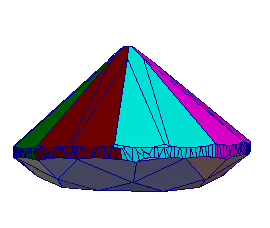
\includegraphics[clip,width=50mm]{allfinal1.png}          
}		
	\caption{lexus 400c Wol 1}
	\label{allfinal1}
	\newpage
\noindent\centering{
    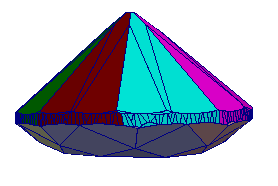
\includegraphics[clip,width=55mm]{allfinal2.png}
}		
	\caption{lexus 400c wol 2}
	\label{allfinal2}

\noindent\centering{
    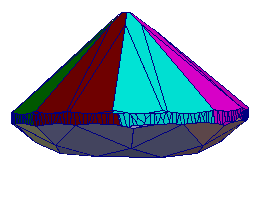
\includegraphics[clip,width=50mm]{allfinal3.png}
}		
	\caption{lexus 400c wol 3}
	\label{allfinal3}
\end{multicols}
\end{figure}

\newpage
\noindent 
Вывод программы повторной кластеризации при начальном пороге 0.5:\\
==========  Clusterization for 1 ==============\\
cluster0 = \{0, 77, 146, 179, 224, 259, ; area = 0.984734\}\\
cluster1 = \{1, 73, 148, 153, 210, 238, ; area = 1.049154\}\\
cluster2 = \{71, 105, 135, 160, 166, 200, 220, 228, 232, ; area = 0.249113\}\\
cluster3 = \{3, 22, 23, 72, 76, 82, 90, 101, 115, 116, 131, 138, 144, 174, 176, 186, 216, 219, 222, 229, 242, 253, 255, 261, 281, ; area = 6.932581\}\\
cluster4 = \{4, 24, 25, 57, 63, 68, 86, 89, 100, 109, 113, 117, 118, 145, 151, 154, 155, 161, 164, 168, 170, 183, 194, 197, 199, 223, 227, 240, 245, 254, 258, 260, 271, 279, 287, 289, ; area = 7.183565\}\\
\textcolor{blue}
{
cluster5 = \{5, 26, 27, 65, 75, 80, 91, 98, 110, 121, 124, 127, 133, 141, 149, 158, 171, 173, 189, 193, 196, 211, 212, 213, 214, 215, 218, 230, 246, 248, 277, 278, ; area = 7.492867\}\\
}
cluster6 = \{6, 28, 29, 59, 61, 64, 70, 78, 88, 95, 97, 108, 122, 126, 137, 140, 159, 163, 178, 181, 188, 195, 198, 208, 209, 235, 249, 251, 257, 262, 270, 273, 274, 283, 285, ; area = 6.629843\}\\
cluster7 = \{7, 30, 31, 58, 60, 74, 84, 93, 103, 106, 111, 125, 142, 143, 152, 157, 165, 167, 185, 201, 205, 217, 221, 233, 237, 241, 256, 263, 266, 282, 284, 286, ; area = 6.951828\}\\
cluster8 = \{8, 32, 33, 55, 292, ; area = 3.778276\}\\
cluster9 = \{9, 34, 35, 49, ; area = 3.942000\}\\
cluster10 = \{10, 36, 37, 50, 290, ; area = 3.691137\}\\
cluster11 = \{11, 38, 39, ; area = 2.833495\}\\
cluster12 = \{12, 40, 41, 42, 51, 52, 291, ; area = 5.530629\}\\
cluster13 = \{48, ; area = 0.745330\}\\
cluster14 = \{13, 14, 43, 44, 45, 53, 54, 56, 288, ; area = 19.353001\}\\
cluster15 = \{15, 46, 47, ; area = 2.735335\}\\
cluster16 = \{16, 69, 79, 96, 99, 129, 132, 134, 184, 202, 203, 226, 236, 264, 269, ; area = 3.207922\}\\
cluster17 = \{17, 67, 92, 119, 120, 136, 172, 175, 192, 207, 250, ; area = 2.799638\}\\
cluster18 = \{18, 81, 94, 128, 130, 180, 204, 206, 225, 234, 247, ; area = 3.125138\}\\
cluster19 = \{19, 62, 87, 112, 169, 177, 182, 267, 272, 276, 280, ; area = 2.964616\}\\
cluster20 = \{2, 20, 66, 83, 104, 107, 139, 147, 150, 156, 191, 231, 239, 243, 252, 275, ; area = 3.761505\}\\
cluster21 = \{21, 85, 102, 114, 123, 162, 187, 190, 244, 265, 268, ; area = 2.796126\}\\
allarea = 98.737832\\
==========  Clusterization for 2 ==============\\
cluster0 = \{0, 77, 130, 184, 188, 216, ; area = 0.981934\}\\
cluster1 = \{1, 73, 134, 168, 194, 218, ; area = 1.059479\}\\
cluster2 = \{71, 104, 140, 153, 154, 207, 208, 228, 278, ; area = 0.235695\}\\
cluster3 = \{3, 22, 23, 72, 76, 82, 90, 113, 115, 126, 139, 142, 162, 185, 196, 201, 202, 204, 233, 234, 242, 254, 255, 268, 284, ; area = 6.924241\}\\
cluster4 = \{4, 24, 25, 57, 63, 68, 86, 87, 108, 111, 116, 120, 127, 133, 145, 163, 164, 166, 167, 178, 180, 209, 220, 229, 230, 247, 252, 261, 263, 266, 282, 290, 293, ; area = 7.153783\}\\
\textcolor{blue}
{
cluster5 = \{5, 26, 27, 64, 75, 81, 91, 100, 101, 110, 121, 124, 128, 150, 152, 155, 160, 169, 174, 175, 176, 191, 192, 193, 237, 238, 248, 256, 257, 265, 267, 277, 280, 281, 288, 292, ; area = 7.529387\}\\
}
cluster6 = \{6, 28, 29, 59, 60, 61, 65, 69, 79, 88, 96, 98, 114, 117, 132, 137, 146, 151, 161, 181, 183, 190, 200, 205, 206, 212, 213, 224, 235, 239, 253, 270, 272, 275, 276, 285, 287, ; area = 6.632527\}\\
cluster7 = \{7, 30, 31, 58, 74, 84, 92, 103, 106, 112, 123, 141, 149, 156, 157, 170, 179, 186, 199, 214, 219, 223, 236, 251, 258, 260, 271, 279, 286, 289, ; area = 6.960272\}\\
cluster8 = \{8, 32, 33, 55, 295, ; area = 3.776520\}\\
cluster9 = \{9, 34, 35, 49, ; area = 3.941691\}\\
cluster10 = \{10, 36, 37, 50, 296, ; area = 3.691819\}\\
cluster11 = \{11, 38, 39, ; area = 2.833087\}\\
cluster12 = \{12, 40, 41, 42, 51, 52, 291, ; area = 5.543814\}\\
cluster13 = \{48, ; area = 0.744224\}\\
cluster14 = \{13, 14, 43, 44, 45, 53, 54, 56, 294, ; area = 19.336340\}\\
cluster15 = \{15, 46, 47, ; area = 2.736993\}\\
cluster16 = \{16, 70, 78, 95, 97, 129, 131, 135, 197, 203, 211, 227, 231, 232, ; area = 3.196353\}\\
cluster17 = \{17, 67, 93, 118, 122, 147, 182, 187, 215, 217, 269, ; area = 2.808577\}\\
cluster18 = \{18, 80, 94, 99, 125, 138, 173, 189, 210, 222, 225, 262, ; area = 3.129662\}\\
cluster19 = \{19, 62, 89, 119, 171, 172, 177, 241, 259, 283, ; area = 2.945934\}\\
cluster20 = \{2, 20, 66, 83, 102, 107, 143, 144, 148, 159, 198, 226, 240, 244, 245, 246, 264, 273, ; area = 3.741092\}\\
cluster21 = \{21, 85, 105, 109, 136, 158, 165, 195, 221, 243, 249, 250, 274, ; area = 2.833236\}\\
allarea = 98.736659\\
\newpage
==========  Clusterization for 3 ==============\\
cluster0 = \{0, 76, 129, 170, 181, 258, 266, 275, ; area = 0.987085\}\\
cluster1 = \{1, 72, 128, 154, 189, 236, ; area = 1.060255\}\\
cluster2 = \{70, 103, 135, 153, 163, 183, 216, 225, 244, 250, 273, ; area = 0.255731\}\\
cluster3 = \{3, 22, 23, 71, 75, 80, 89, 99, 115, 120, 130, 136, 142, 166, 176, 186, 195, 209, 221, 230, 238, 259, 260, 272, 281, 290, 292, ; area = 6.914082\}\\
cluster4 = \{4, 24, 25, 57, 62, 67, 84, 86, 105, 107, 109, 119, 131, 132, 151, 156, 160, 165, 177, 180, 187, 188, 192, 204, 214, 220, 226, 243, 254, 289, 298, ; area = 7.156528\}\\
\textcolor{blue}
{
cluster5 = \{5, 26, 27, 63, 74, 79, 87, 96, 98, 113, 114, 124, 127, 138, 139, 152, 158, 171, 173, 175, 197, 199, 202, 211, 213, 218, 222, 224, 235, 241, 253, 262, 265, 267, 271, 278, 286, 288, ; area = 7.490189\}\\
}
cluster6 = \{6, 28, 29, 58, 59, 60, 64, 68, 77, 94, 95, 110, 117, 125, 141, 143, 157, 169, 172, 178, 191, 194, 198, 203, 215, 219, 231, 242, 249, 263, 274, 293, 294, 295, ; area = 6.649838\}\\
cluster7 = \{7, 30, 31, 73, 81, 88, 100, 104, 116, 121, 137, 146, 147, 150, 155, 161, 182, 207, 210, 223, 227, 233, 237, 245, 251, 255, 269, 276, 291, ; area = 6.924438\}\\
cluster8 = \{8, 32, 33, 55, 302, ; area = 3.779985\}\\
cluster9 = \{9, 34, 35, 49, ; area = 3.940620\}\\
cluster10 = \{10, 36, 37, 50, ; area = 3.676376\}\\
cluster11 = \{11, 38, 39, ; area = 2.833928\}\\
cluster12 = \{12, 40, 41, 42, 51, 52, 297, ; area = 5.549255\}\\
cluster13 = \{48, ; area = 0.744159\}\\
cluster14 = \{13, 14, 43, 44, 45, 53, 54, 56, 299, 300, ; area = 19.356865\}\\
cluster15 = \{15, 46, 47, ; area = 2.734612\}\\
cluster16 = \{16, 69, 78, 91, 93, 123, 126, 145, 184, 200, 205, 206, 229, 240, 246, 280, 296, ; area = 3.221952\}\\
cluster17 = \{17, 66, 90, 118, 122, 140, 179, 185, 212, 247, 270, 279, ; area = 2.773333\}\\
cluster18 = \{18, 92, 97, 133, 148, 174, 190, 193, 196, 252, 261, 285, ; area = 3.126491\}\\
cluster19 = \{19, 61, 85, 111, 112, 159, 168, 232, 234, 248, 284, 287, ; area = 2.987012\}\\
cluster20 = \{2, 20, 65, 82, 102, 108, 134, 149, 162, 167, 201, 228, 264, 277, 282, 283, ; area = 3.748960\}\\
cluster21 = \{21, 83, 101, 106, 144, 164, 208, 217, 239, 256, 257, 268, 301, ; area = 2.818898\}\\
allarea = 98.730593
\begin{center}
S12 = 0.000250\;\;\;\;\;
S13 = 0.000230\;\;\;\;\;
S23 = 0.000374
\end{center}
\begin{figure}[h]
\noindent\centering{
    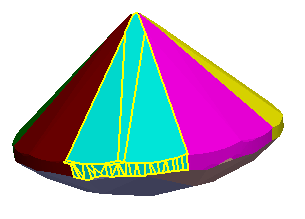
\includegraphics[clip,width=60mm]{rund.png}
          }
\caption{Слияние больших кластеров.}
\label{rund}
\end{figure}
\newpage



После того, как мы разбили многогранники на одинаковое число кластеров можно видеть следующую картину. 
Кластеры образуют на многогранниках соответствующие друг другу структуры. На каждом из многогранников,
например образовалось скопление граней в  которое вошли боковые грани и часть рундиста. На Рис.\ref{rund}
выделен кластер №5. Его грани окрашены голубым цветом, а ребра желтым. В выводе программы 
номера граней, входящих в кластер №5 выделены голубым цветом у каждого многогранника. 

В каждом из многогранников у кластера №5 разное количество граней, но похожий вес. Такое происходит 
из за того, что в рундисте большое количество граней, эти грани так или иначе примыкают  к кластерам, образуя 
такого рода погрешность. Но маленькие грани не меняют общей картины, об этом говорит то, что 
попарно вычисленная величина $S_{ij}$ мала для любых двух из  трех рассмотренных многогранников.  
Для двух многогранников такое сходство говорит, что это или модели очень похожих драгоценных камней, или это
две модели одного и того же камня.  
\newpage
\section{Заключение}
Перед нами стояла задача выбрать для многогранника систему координат,  в которой он примет стандартное положение для 
возможности дальнейшего сравнения многогранников.

Описанные алгоритмы были разработаны  с использованием средств математического, функционального, 
кластерного анализа и механики твердого тела. 
 
Начальными данными описанных алгоритмов были координаты вершин многогранников, уравнения граней и списки вершин, 
лежащих в каждой из граней многогранника.

Из геометрических характеристик мы выделили точечные, поверхностные и объемные. С помощью объемных характеристик 
была выбрана система координат для многогранника, в которой он принял свое стандартное положение.

Далее было проведено сравнение многогранников, находящихся в стандартном положении.

Перед сравнением многогранников была проведена коррекция их теневых контуров.  
Она проводится прежде всего, чтобы убедиться, что угол поворота многогранников друг относительно друга очень маленький.
Нам нужно убедиться, что многогранники хорошо слились в стандартном положении. Об этом говорит использованная в алгоритме
коррекции норма $\Phi(\alpha)$.

После коррекции их положения, с помощью поверхностных характеристик был разработан принцип, по которому 
мы научились сравнивать многогранники, находящиеся в стандартном положении.

Все описанные в работе алгоритмы были применены на практике как на искусственно созданных, 
так и на реальных моделях. 

Программы, вывод которых приводился в работе, были написаны на языке C++, визуализация моделей
проводилась при помощи программ ParaView 3.8.0  и Advanced Grapher 2.2. 

Данные методы могут служить  автоматизации составления документации для драгоценных камней и 
для их классификации, т.к. с помощью этих методов можно ставить камни в стандартное положение 
и делать выводы о том  на сколько они похожи.

\newpage
\begin{thebibliography}{99}                    % Список литературы
\addcontentsline{toc}{section}{Список литературы}

\bibitem{kolm}
А.Н.Колмогоров, С.В.Фомин Элементы теории функций и функционального анализа. М.:Наука, 1976. 411с.

\bibitem{zor}
В.А.Зорич  Математический анализ Ч.II. M.:Наука, 1984. 229c.

\bibitem{vilke}
В.Г.Вильке Теоретическая механика. М.: Изд-во МГУ, 1998. 115с.

\bibitem{Epif}
В.И.Епифанов, А.Я.Песина, Л.В.Зыков Технология обработки алмазов в бриллианты. M.: Высш. шк., 1987. 196с.

\bibitem{wiki-ogranka}
\textit{Википедия. Свободная энциклопедия.} Огранка\\
(http://ru.wikipedia.org/wiki/Огранка)


\bibitem{mink}
Г.Минковский Общие теоремы о выпуклых многогранниках, УМН, 1936, № 2, 55–71


\bibitem{mand}
И.Д.Мандель Кластерный анализ. М.:Финансы и статистика, 1988, 39с. 

\bibitem{prep}
Ф.Препарата, М.Шеймос  Вычислительная геометрия:введение. М.:Мир, 1989, 215c


\bibitem{3dbook} 
OctoNus Software Ltd, 3D-book
http://3dbook.octonus.com/data/3dbook.html


\bibitem{hier}
Székely, G. J. and Rizzo, M. L. (2005) Hierarchical clustering via Joint Between-Within Distances: Extending Ward's Minimum Variance Method, Journal of Classification 22, 151-183.


\end{thebibliography}


\end{document}



